%  LaTeX support: latex@mdpi.com 
%  For support, please attach all files needed for compiling as well as the log file, and specify your operating system, LaTeX version, and LaTeX editor.

%=================================================================
\documentclass[journal,article,submit,pdftex,moreauthors]{Definitions/mdpi} 
% For posting an early version of this manuscript as a preprint, you may use "preprints" as the journal and change "submit" to "accept". The document class line would be, e.g., \documentclass[preprints,article,accept,moreauthors,pdftex]{mdpi}. This is especially recommended for submission to arXiv, where line numbers should be removed before posting. For preprints.org, the editorial staff will make this change immediately prior to posting.

%--------------------
% Class Options:
%--------------------
%----------
% journal
%----------
% Choose between the following MDPI journals:
% acoustics, actuators, addictions, admsci, adolescents, aerospace, agriculture, agriengineering, agronomy, ai, algorithms, allergies, alloys, analytica, animals, antibiotics, antibodies, antioxidants, applbiosci, appliedchem, appliedmath, applmech, applmicrobiol, applnano, applsci, aquacj, architecture, arts, asc, asi, astronomy, atmosphere, atoms, audiolres, automation, axioms, bacteria, batteries, bdcc, behavsci, beverages, biochem, bioengineering, biologics, biology, biomass, biomechanics, biomed, biomedicines, biomedinformatics, biomimetics, biomolecules, biophysica, biosensors, biotech, birds, bloods, blsf, brainsci, breath, buildings, businesses, cancers, carbon, cardiogenetics, catalysts, cells, ceramics, challenges, chemengineering, chemistry, chemosensors, chemproc, children, chips, cimb, civileng, cleantechnol, climate, clinpract, clockssleep, cmd, coasts, coatings, colloids, colorants, commodities, compounds, computation, computers, condensedmatter, conservation, constrmater, cosmetics, covid, crops, cryptography, crystals, csmf, ctn, curroncol, currophthalmol, cyber, dairy, data, dentistry, dermato, dermatopathology, designs, diabetology, diagnostics, dietetics, digital, disabilities, diseases, diversity, dna, drones, dynamics, earth, ebj, ecologies, econometrics, economies, education, ejihpe, electricity, electrochem, electronicmat, electronics, encyclopedia, endocrines, energies, eng, engproc, ent, entomology, entropy, environments, environsciproc, epidemiologia, epigenomes, est, fermentation, fibers, fintech, fire, fishes, fluids, foods, forecasting, forensicsci, forests, foundations, fractalfract, fuels, futureinternet, futureparasites, futurepharmacol, futurephys, futuretransp, galaxies, games, gases, gastroent, gastrointestdisord, gels, genealogy, genes, geographies, geohazards, geomatics, geosciences, geotechnics, geriatrics, hazardousmatters, healthcare, hearts, hemato, heritage, highthroughput, histories, horticulturae, humanities, humans, hydrobiology, hydrogen, hydrology, hygiene, idr, ijerph, ijfs, ijgi, ijms, ijns, ijtm, ijtpp, immuno, informatics, information, infrastructures, inorganics, insects, instruments, inventions, iot, j, jal, jcdd, jcm, jcp, jcs, jdb, jeta, jfb, jfmk, jimaging, jintelligence, jlpea, jmmp, jmp, jmse, jne, jnt, jof, joitmc, jor, journalmedia, jox, jpm, jrfm, jsan, jtaer, jzbg, kidney, kidneydial, knowledge, land, languages, laws, life, liquids, literature, livers, logics, logistics, lubricants, lymphatics, machines, macromol, magnetism, magnetochemistry, make, marinedrugs, materials, materproc, mathematics, mca, measurements, medicina, medicines, medsci, membranes, merits, metabolites, metals, meteorology, methane, metrology, micro, microarrays, microbiolres, micromachines, microorganisms, microplastics, minerals, mining, modelling, molbank, molecules, mps, msf, mti, muscles, nanoenergyadv, nanomanufacturing, nanomaterials, ncrna, network, neuroglia, neurolint, neurosci, nitrogen, notspecified, nri, nursrep, nutraceuticals, nutrients, obesities, oceans, ohbm, onco, oncopathology, optics, oral, organics, organoids, osteology, oxygen, parasites, parasitologia, particles, pathogens, pathophysiology, pediatrrep, pharmaceuticals, pharmaceutics, pharmacoepidemiology, pharmacy, philosophies, photochem, photonics, phycology, physchem, physics, physiologia, plants, plasma, pollutants, polymers, polysaccharides, poultry, powders, preprints, proceedings, processes, prosthesis, proteomes, psf, psych, psychiatryint, psychoactives, publications, quantumrep, quaternary, qubs, radiation, reactions, recycling, regeneration, religions, remotesensing, reports, reprodmed, resources, rheumato, risks, robotics, ruminants, safety, sci, scipharm, seeds, sensors, separations, sexes, signals, sinusitis, skins, smartcities, sna, societies, socsci, software, soilsystems, solar, solids, sports, standards, stats, stresses, surfaces, surgeries, suschem, sustainability, symmetry, synbio, systems, taxonomy, technologies, telecom, test, textiles, thalassrep, thermo, tomography, tourismhosp, toxics, toxins, transplantology, transportation, traumacare, traumas, tropicalmed, universe, urbansci, uro, vaccines, vehicles, venereology, vetsci, vibration, viruses, vision, waste, water, wem, wevj, wind, women, world, youth, zoonoticdis 
\usepackage{siunitx}
\usepackage{eurosym}
\usepackage{xcolor}
\usepackage{units}
\DeclareSIUnit{\pers}{pers}
\usepackage{footnote}

\usepackage{csquotes}
\makesavenoteenv{tabular}
\usepackage{textcomp}
\usepackage[final]{changes}
\DeclareSIUnit{\EUR}{\text{\euro}}
\sisetup{
  per-mode = fraction,
  inter-unit-product = \ensuremath{{}\cdot{}},
}
% \setlength{\arrayrulewidth}{1mm}
% \setlength{\tabcolsep}{18pt}
% \renewcommand{\arraystretch}{2.5}
% \newcolumntype{s}{>{\columncolor[HTML]{AAACED}} p{3cm}}
% \arrayrulecolor[HTML]{DB5800}
%---------
% article
%---------
% The default type of manuscript is "article", but can be replaced by: 
% abstract, addendum, article, book, bookreview, briefreport, casereport, comment, commentary, communication, conferenceproceedings, correction, conferencereport, entry, expressionofconcern, extendedabstract, datadescriptor, editorial, essay, erratum, hypothesis, interestingimage, obituary, opinion, projectreport, reply, retraction, review, perspective, protocol, shortnote, studyprotocol, systematicreview, supfile, technicalnote, viewpoint, guidelines, registeredreport, tutorial
% supfile = supplementary materials

%----------
% submit
%----------
% The class option "submit" will be changed to "accept" by the Editorial Office when the paper is accepted. This will only make changes to the frontpage (e.g., the logo of the journal will get visible), the headings, and the copyright information. Also, line numbering will be removed. Journal info and pagination for accepted papers will also be assigned by the Editorial Office.

%------------------
% moreauthors
%------------------
% If there is only one author the class option oneauthor should be used. Otherwise use the class option moreauthors.

%---------
% pdftex
%---------
% The option pdftex is for use with pdfLaTeX. If eps figures are used, remove the option pdftex and use LaTeX and dvi2pdf.

%=================================================================
% MDPI internal commands
\firstpage{1} 
\makeatletter 
\setcounter{page}{\@firstpage} 
\makeatother
\pubvolume{1}
\issuenum{1}
\articlenumber{0}
\pubyear{2022}
\copyrightyear{2022}
%\externaleditor{Academic Editor: Firstname Lastname} % For journal Automation, please change Academic Editor to "Communicated by"
\datereceived{} 
\dateaccepted{} 
\datepublished{} 
%\datecorrected{} % Corrected papers include a "Corrected: XXX" date in the original paper.
%\dateretracted{} % Corrected papers include a "Retracted: XXX" date in the original paper.
\hreflink{https://doi.org/} % If needed use \linebreak
%\doinum{}
%------------------------------------------------------------------
% The following line should be uncommented if the LaTeX file is uploaded to arXiv.org
%\pdfoutput=1

%=================================================================
% Add packages and commands here. The following packages are loaded in our class file: fontenc, inputenc, calc, indentfirst, fancyhdr, graphicx, epstopdf, lastpage, ifthen, lineno, float, amsmath, setspace, enumitem, mathpazo, booktabs, titlesec, etoolbox, tabto, xcolor, soul, multirow, microtype, tikz, totcount, changepage, attrib, upgreek, cleveref, amsthm, hyphenat, natbib, hyperref, footmisc, url, geometry, newfloat, caption

%=================================================================
%% Please use the following mathematics environments: Theorem, Lemma, Corollary, Proposition, Characterization, Property, Problem, Example, ExamplesandDefinitions, Hypothesis, Remark, Definition, Notation, Assumption
%% For proofs, please use the proof environment (the amsthm package is loaded by the MDPI class).

%=================================================================
% Full title of the paper (Capitalized)
\Title{Minimum-cost fast-charging infrastructure planning for electric vehicles along the Austrian high-level road network}

% MDPI internal command: Title for citation in the left column
\TitleCitation{Minimum-cost fast-charging infrastructure planning for electric vehicles along the Austrian high-level road network}

% Author Orchid ID: enter ID or remove command
\newcommand{\orcidauthorA}{0000-0001-9307-6669} % Add \orcidA{} behind the author's name
\newcommand{\orcidauthorB}{0000-0002-8599-6278} % Add \orcidB{} behind the author's name
\newcommand{\orcidauthorC}{0000-0002-9111-9941} % Add \orcidB{} behind the author's name

% Authors, for the paper (add full first names)
\Author{Antonia Golab $^{1}$*\orcidA{}, Sebastian Zwickl-Bernhard $^{1}$\orcidB{}  and Hans Auer $^{1}$ \orcidC{}}

%\longauthorlist{yes}

% MDPI internal command: Authors, for metadata in PDF
\AuthorNames{Antonia Golab, Sebastian Zwickl-Bernhard, Hans Auer}

% MDPI internal command: Authors, for citation in the left column
\AuthorCitation{Golab, A.; Zwickl-Bernhard, S.;}
% If this is a Chicago style journal: Lastname, Firstname, Firstname Lastname, and Firstname Lastname.

% Affiliations / Addresses (Add [1] after \address if there is only one affiliation.)
\address{%
$^{1}$ \quad Energy Economy Group (EEG), Technische Universität Wien, Gusshausstraße 25-2\replaced{9}{0}, E370-3, 1040 Vienna, Austria}\\
% $^{2}$ \quad Affiliation 2; e-mail@e-mail.com}

% Contact information of the corresponding author
\corres{Correspondence: golab@eeg.tuwien.at}

% Current address and/or shared authorship
% \firstnote{Current address: Affiliation 3} 
% \secondnote{These authors contributed equally to this work.}
% The commands \thirdnote{} till \eighthnote{} are available for further notes
\usepackage{amsmath}
\usepackage{siunitx}
\usepackage{eurosym}
\usepackage{eurosym}

\DeclareSIUnit{\pers}{pers}
\DeclareSIUnit{\EUR}{\text{\euro}}
\sisetup{
  per-mode = fraction,
  inter-unit-product = \ensuremath{{}\cdot{}},
}
%\simplesumm{} % Simple summary

%\conference{} % An extended version of a conference paper

% Abstract (Do not insert blank lines, i.e. \\) 
% \abstract{A single paragraph of about 200 words maximum. For research articles, abstracts should give a pertinent overview of the work. We strongly encourage authors to use the following style of structured abstracts, but without headings: (1) Background: place the question addressed in a broad context and highlight the purpose of the study; (2) Methods: describe briefly the main methods or treatments applied; (3) Results: summarize the article's main findings; (4) Conclusion: indicate the main conclusions or interpretations. The abstract should be an objective representation of the article, it must not contain results which are not presented and substantiated in the main text and should not exaggerate the main conclusions.}
\abstract{Given the on-going transformation of the transport sector toward electrification, expansion of the current charging infrastructure is essential to meet future charging demands. The lack of fast-charging infrastructure along highways and motorways is a particular obstacle for long-distance travel with battery-electric vehicles (BEVs). In this context, we propose a charging infrastructure allocation model that allocates and sizes fast-charging stations along high-level road networks while minimizing the costs for infrastructure investment. The modeling framework is applied to the Austrian highway and motorway network, and the needed expansion of the current fast-charging infrastructure in place is modeled under different future scenarios for 2030. Within these, the share of BEVs in the car fleet, developments in BEV technology and road traffic load changing in the face of future modal shift effects are altered. In particular, we analyze the change in the requirements for fast-charging infrastructure in response to enhanced driving range and growing BEV fleet. The results indicate that improvements in the driving range of BEVs will have limited impact and hardly affect future costs of the expansion of the fast-charging infrastructure. On the contrary, the improvements in the charging power of BEVs have the potential to reduce future infrastructure costs.}



% Keywords
\keyword{fast-charging; placement and sizing of charging stations; highway charging infrastructure; long-distance travel; battery-electric vehicles; optimization model; Austrian road network} 

% The fields PACS, MSC, and JEL may be left empty or commented out if not applicable
%\PACS{J0101}
%\MSC{}
%\JEL{}

%%%%%%%%%%%%%%%%%%%%%%%%%%%%%%%%%%%%%%%%%%
% Only for the journal Diversity
%\LSID{\url{http://}}

%%%%%%%%%%%%%%%%%%%%%%%%%%%%%%%%%%%%%%%%%%
% Only for the journal Applied Sciences:
%\featuredapplication{Authors are encouraged to provide a concise description of the specific application or a potential application of the work. This section is not mandatory.}
%%%%%%%%%%%%%%%%%%%%%%%%%%%%%%%%%%%%%%%%%%

%%%%%%%%%%%%%%%%%%%%%%%%%%%%%%%%%%%%%%%%%%
% Only for the journal Data:
%\dataset{DOI number or link to the deposited data set in cases where the data set is published or set to be published separately. If the data set is submitted and will be published as a supplement to this paper in the journal Data, this field will be filled by the editors of the journal. In this case, please make sure to submit the data set as a supplement when entering your manuscript into our manuscript editorial system.}

%\datasetlicense{license under which the data set is made available (CC0, CC-BY, CC-BY-SA, CC-BY-NC, etc.)}

%%%%%%%%%%%%%%%%%%%%%%%%%%%%%%%%%%%%%%%%%%
% Only for the journal Toxins
%\keycontribution{The breakthroughs or highlights of the manuscript. Authors can write one or two sentences to describe the most important part of the paper.}

%%%%%%%%%%%%%%%%%%%%%%%%%%%%%%%%%%%%%%%%%%
% Only for the journal Encyclopedia
%\encyclopediadef{Instead of the abstract}
%\entrylink{The Link to this entry published on the encyclopedia platform.}
%%%%%%%%%%%%%%%%%%%%%%%%%%%%%%%%%%%%%%%%%%
\begin{document}

%%%%%%%%%%%%%%%%%%%%%%%%%%%%%%%%%%%%%%%%%%
% \setcounter{section}{-1} %% Remove this when starting to work on the template.
% \section{How to Use this Template}

% The template details the sections that can be used in a manuscript. Note that the order and names of article sections may differ from the requirements of the journal (e.g., the positioning of the Materials and Methods section). Please check the instructions on the authors' page of the journal to verify the correct order and names. For any questions, please contact the editorial office of the journal or support@mdpi.com. For LaTeX-related questions please contact latex@mdpi.com.%\endnote{This is an endnote.} % To use endnotes, please un-comment \printendnotes below (before References). Only journal Laws uses \footnote.

% The order of the section titles is: Introduction, Materials and Methods, Results, Discussion, Conclusions for these journals: aerospace,algorithms,antibodies,antioxidants,atmosphere,axioms,biomedicines,carbon,crystals,designs,diagnostics,environments,fermentation,fluids,forests,fractalfract,informatics,information,inventions,jfmk,jrfm,lubricants,neonatalscreening,neuroglia,particles,pharmaceutics,polymers,processes,technologies,viruses,vision


\section{Introduction}

% BEVs
Currently, 10\% of the global GHG emissions are traced back to the transport sector, and 45\% of these are caused by passenger road transport \citep{cazzola2016global}. The global transport demand is expected to significantly grow in the upcoming decades due to rising incomes in developing countries and infrastructure development \citep{Moriarty2008}. One of the key measures against the growth of thereto related GHG emission\added{s} by the motorized passenger transport is the introduction of battery-electric vehicles (BEVs). This technology has several advantages --- in contrast to vehicles with internal combustion engines (ICE) --- including the absence of tailpipe emissions, significantly higher energy efficiency, positive impact on air quality in urban areas, and lower noise pollution \cite{wevj8040996}. However, the market penetration of BEVs significantly varies among countries \cite{Parliament2018}; one of the most prominent role models is Norway which is the front runner of new registrations of electric vehicles, as in Norway, 60\% of newly registered passenger cars are exclusively powered by an electric engine \citep{stat}. According to the Paris Agreement, 20\% of the global passenger car fleet must be electric engine-powered by 2030 \cite{paris}. Globally, the market share of electric vehicles is currently 5\% and there are 10 Mio. electric vehicles in the global passenger car fleet, which has the size of around one billion \cite{cazzola2016global}.   

% Austrian case study 
In Austria, BEVs currently account for $1.5\%$ of the total passenger car fleet \cite{beoe}. The Austrian government has pledged to climate neutrality until 2040, and a document outlining the decarbonization path for the transport network was recently released, called \enquote{Austria's Mobility Plan 2030} \cite{Nachhaltig}. In this document, it is specified that climate change mitigation in the passenger transport sector will be achieved by means of electromobility in the passenger car fleet, a shift to low-carbon modes and travel avoidance. One focal point of the described pathway to decarbonization is the enablers of the transition to green mobility, which are technological developments and infrastructure adoption --- the latter includes charging infrastructure. 

% charging infrastructure
Along the road to 100\% electromobility, the phenomenon of \textit{range anxiety}\footnote{\textit{Range anxiety} describes the fear of not being able to continue a trip due to the limited driving range of a BEV and missing charging infrastructure.} is considered to be one of the most prominent impediments for the adoption of BEVs. Furthermore, the long charging duration causes many potential buyers to decide against the purchase of a BEV \citep{Coffman2017, Efe2018}. These technological aspects of BEVs have significantly improved over the last years, and industry has been working on battery technology solutions, which could further increase the driving range and charging speed of BEVs \citep{IRENA2019, Thielmann2017}. Complementary to this, the deployment of fast-charging infrastructure plays a significant role in the BEV adoption. If sufficiently allocated, such infrastructure can work as a safety net to counteract range anxiety and enable fast-charging processes \citep{Neaimeh2017}. The expansion of fast-charging infrastructure along high-level road networks has also been the focus of many governments in EU countries \citep{Parliament2018}. Moreover, the aimed expansion has been formulated in the recently published policy package \enquote{Fit for 55} \citep{fit455}, wherein it is specified that a charging station should be available at least every $60km$ along the Trans-European Transport Network until 2030.

% model and input parameters 
The key objective of this work is to present a novel model approach for highway charging infrastructure design, which determines the cost-optimal position and, simultaneously, the sizing of charging stations with regard to the demand given by long-distance BEV drivers traveling. Another goal is to quantify the needed future expansion of the fast-charging infrastructure that is currently in place and, within this, to understand how the share of BEVs, changes in overall road traffic load, and technological advancements of BEVs affect this future projection. The analyses are conducted based on the model application to the Austrian highway network\footnote{This also includes motorways. For better readability of this paper, the phrase of \textit{highway} is used for both, highways and motorways, in the street network.} for 2030. The deduced findings of this work aim to support policy-makers in their investment decisions associated with the development of a demand-oriented fast-charging infrastructure.
% Against this background, we propose a modeling framework which determines the optimal allocation and sizing of charging stations i. This is applied to the Austrian highway network\ Under four different climate change mitigation scenarios, among which share of BEVs, road traffic load and technological advancements are varied, a cost-minimum expansion of the fast-charging infrastructure for the year 2030 is modeled. In further analysis, the impact by increasing BEV share and driving range on the infrastructure costs are analyzed in order to gain insight into their interaction and deduce findings which could support policy-makers in investment decisions.
% The proposed modeling framework can be applied to different high-level road networks of different extent and allocation and can give insight into required charging infrastructure depending on different technological attributes of the BEV, BEV fleet and traffic loads.


% The market penetration of BEVs has risen by \hl{...} since rein
% \begin{itemize}
%     \item Policies related to decarbonization of transport sector (Fit for 55, green deal, "Mobilitätsmasterplan 2030") 
%     \item electrification of passenger sector
%     \item importance of decarbonization of transport sector in Austria
%     \item development of a charging infrastructure to promote BEV usage (reducing range anxiety)
%     \item Climate mitigation paths in the transport sector (increasing energy efficiency, electrification, modal shift)
%     \item \citet{Baumgarte2021}
%     \item range anxiety, long charging processes and limited range are among the core issues in EV adoption
%     \item therefore, the appropriate spatial distribution of fast-charging infrastructure is of importance 
% \end{itemize}
% Similar as in the study by \citet{Jochem2016}, we assume that plug-in hybrid electric vehicles rather refuel their conventional engine on long-distance trips rather than recharge the electric one for convenience. 



%The introduction should briefly place the study in a broad context and highlight why it is important. It should define the purpose of the work and its significance. The current state of the research field should be reviewed carefully and key publications cited. Please highlight controversial and diverging hypotheses when necessary. Finally, briefly mention the main aim of the work and highlight the principal conclusions. As far as possible, please keep the introduction comprehensible to scientists outside your particular field of research. Citing a journal paper \cite{ref-journal}. Now citing a book reference \cite{ref-book1,ref-book2} or other reference types \cite{ref-unpublish,ref-communication,ref-proceeding}. Please use the command \citep{ref-thesis,ref-url} for the following MDPI journals, which use author--date citation: Administrative Sciences, Arts, Econometrics, Economies, Genealogy, Humanities, IJFS, Journal of Intelligence, Journalism and Media, JRFM, Languages, Laws, Religions, Risks, Social Sciences, Literature.
%%%%%%%%%%%%%%%%%%%%%%%%%%%%%%%%%%%%%%%%%%
\section{Related Work}

    % \subsection{Charging along highways/DCFC charging}
    
    % where needed, technolog. developments, short: on-going projects (Europe, Austria)
    
    
    % \subsection{Charging station allocation modelling}
    % review on Charging station allocation modelling

    \subsection{Climate change mitigation in the passenger transport sector}
Essentially, there are four main potential drivers to counteract increasing GHG emissions in the face of rising travel demand, namely: avoidance of journeys, shift to low-carbon modes, fuel substitution, and improvements in energy efficiency \citep{Josefina, Edelenbosch2017, Milovanoff2021}. These drivers are deeply intertwined, and their effectiveness is rooted in technological progress, social learning, and infrastructure adoptions \citep{Edelenbosch2017, Muller2021}. \citet{PRIEMUS2001167} describes the close relationship between people's mobility behavior and spatial infrastructure planning, indicating that modal shift can only happen effectively as a response to changes in transport network infrastructure. The same is highlighted by \citet{briggs2015automotive} who finds that infrastructure planning decisions affect the modal split long-term, for over multiple decades, and can, therefore, also form a macro-level barrier to climate mitigation \citep{UNRUH2000817}. Infrastructure changes supporting climate-friendly mobility include the expansion of the railway system and construction of sidewalks and cycling routes; they are essentially aimed toward a reduction in motorized transport \citep{SONG2017320, Muller2021}. Other motivators in changing mobility behavior include monetary incentives, such as the adjustment of travel costs, costs of vehicle ownership or parking charges \citep{Hammadou2015, Silva2022}. 
% Though, there is still a lack of insight into how motivators induce changes in mobility behavior which brings uncertainty into the estimation of how modal shift will develop \citep{Josefina}. 
    
    To decarbonize the passenger transport sector, the introduction of electromobility plays an important role \citep{HEIDRICH201717, Das2020}. Following the Paris Agreement, the goal is to substitute the passenger car fleet for vehicles with electric engines by 2040 \cite{Nachhaltig}. However, manufacture and end-of-life treatment of electric vehicles require more energy than vehicles powered by diesel or petrol\deleted{.}\added{;} \deleted{L}\added{l}ife cycle assessments revealed that electric vehicles still emit less GHG emissions over the lifetime than internal-combustion-engine (ICE) vehicles \citep{VanVliet2011, Bauer2015}. These life cycle assessments also highlight that the positive effect of electric vehicles is highly dependent on the shares of renewable energy sources in the energy mix; otherwise\added{, so these studies suggest,} the overall emissions can be even higher than those emitted by ICE vehicles when the energy mix is highly dominated by fossil-fuel energy carriers. Electric vehicles are commonly divided into: plug-in electric vehicles (PEVs), plug-in hybrid electric vehicles (PHEVs), BEVs and fuell cell electric vehicles (FCEVs). PEVs encompass PHEVs and BEVs, which can be recharged via a plug at charging stations, unlike HEVs. Currently, HEVs and BEVs together dominate the market of electric vehicles but only BEVs have no tailpipe emissions \citep{VanVliet2011, Ajanovic2015}. 
    
    \citet{Costa2021} found that measures related to behavioral changes, i.e., reduction in activity and change in travel modes, have overall similar potential to technological improvements, i.e., an increase in energy efficiency in private transport and the adoption of low-carbon technologies, in climate change mitigation. \citet{DILLMAN2021102614} argued the same thing based on a study on the decarbonization of the passenger transport sector on the city level. They found that measures of both types together, changes in travel behaviour and technological improvments, are the most effective in the decarbonization of passenger transport.
    
    
    
    
    

    % The substitution of fossil fuels 
    
    % The motivation behind behavioral changes of mode switch or avoidance   
    % \citet{Milovanoff2021} analysed climate migation drivers in passenger transport in the urban context and found that cross-sectoral mitigation efforts such as between the energy sector and passenger transport sector are vital to achieve decarbonization goals, especially in regards to increased energy generation from renewable energy sources and electro-mobility.
    
    %Avoidance of journeys and progressive modal shift is highly dependent on behavioral changes 
    
    
    
    
    % A core challenge in the climate mitigation within this sector is the overall growth in demand which can be traced back to .. and ... . According to the "AR 5 Mitigation of Climate Change" report by IPCC (REF), there are two important drivers: Reduction of usage of fossil-fuel energy through electrification of transport systems and reduction of overall energy demand through shift to energy efficient and low-carbon modes and through improving efficiency in transport systems. Due to the close interaction between available infrastructure and mode choice together with overall transport demand, investments in supporting infrastructure are vital.  

%     Since ... ,  pkm has risen globally and OECD projects to rise up to ... in ..., given the close correlation between a country's GDP and degree of motorization (REF) which poses a major obstacle in climate mitigation in the transport sector (REF low mobility). Though, there are studies reporting a partial decoupling of economic growth and rise in individual vehicle ownership \citep[see e.g.][]{}. Either way, a rise in vehicle ownership is still evident and on-going, especially in non-urban areas ... , while in urban areas such as Vienna, the share of travels by public transports and bikes have risen. This phenomena has been also observed in other major cities, such as ... and .. [REF].   
    
%     Along-side these developments, shifts to more energy-efficient modes has been also evident in increasing sales of BEVs: *Positive example Norway*
%     Europe-wide, ...
    
%     In the recently published "Fit 4 55" package by the European Union, guidelines on charging infrastructure expansion along the TEN-T network are described. 
%     As the Austrian government has pledged carbon neutrality until 2040, 
    
%     According to the Paris agreement, $20\%$ of global car fleet is intended to have an electric engine. Today's share of EVs is about .. \% which indicates that there is a need in substantial market growth. 
    
%     focus of policies: electromobility, Ausbau electrified rail network in order to reduce long-distance travel by car or plane. 
    
%     .. Structural needs to avoid "lock-in" effect and pave a way to decarbonation. 
    
%     "lock-in effect", infrastructure 
    
%     Modal shift, traffic avoidance and technological development 
%     \citet{Muller2021}; Study on needed measures to enable modal shift in Ruhr; indicates that infrastructural changes are important; reduction of car use through e.g. densification of railway stations, new housing around there 
    
%     \citet{Edelenbosch2017} identified increase in energy efficiency and fuel switch to be the main drivers in climate mitigation in the transport sector in IAMs. 
%     \citet{Milovanoff2021} analysed climate migation drivers in passenger transport in the urban context and found that cross-sectoral mitigation efforts such as between the energy sector and passenger transport sector are vital to achieve decarbonization goals, especially in regards to increased energy generation from renewable energy sources and electro-mobility. Energy mix impacts ev \citet{Deetman2015}
    
%     \citet{Deetman2015}: regional dependency of effectiveness of policity incentives
%     modal shift: complex, on high local level, high dependence on structure \citep{Muller2021}
%     \citet{Siskos2015}: large uncertainties for robust policies for 2050; Co2 standards are necessary trigger for wider updtake of EVs 
%     BEVs vs PEVs
    
    
    
%     On the one hand-side, technological improvements ... energy efficiency  
    
%     on the other hand-side, low mobility?
   
    
%   %  two main drivers in the climate mitigation in the passenger transport sector are identified:  Further, 
%     % Though, the issue of increasing transportation demand in face of passenger transport activity which emphasize s the need of long-term infrastructure changes influencing people's choice of mode and transportation demand. 
    
%     % Overall, within various descriptions of mitigation pathways in the passenger transport sector, 
    
    
    
    
    
    
%     \begin{itemize}
%         \item \textbf{Climate mitigation paths:} Decarbonization through alternative fuels, modal shift, potentials in modal shift
%         \item \citet{Edelenbosch2017}: passenger transport futures..., 
%         \item \citet{Santarromana2020}
%         \item  \textbf{Recent Developments considering these different opportunities} Increasing penetration of BEV in market ; \cite{Ajanovic2015}; Recent developments in Modal split (urban versus suburban trends);
%         \item  \textbf{Policy push in EU/Austria} Incentives for EV purchases, Austria's Mobility Master Plan, Green deal, ... \textrightarrow main foci of policies in climate mitigation in passenger transport sector 
%         \item \citet{Georgatzi2020}, \citet{Costa2021}, \citet{Letnik2018}, \citet{Maria2018}, \citet{Hill2019}
%         \item \citet{Dominkovic2018}: electric vehicles; key factor: clean energy 
%         \item strong interaction between infrastructure and passenger transportation 
%     \end{itemize}
  
    
    \subsection{Importance of fast-charging infrastructure}
    
    % dramaturgie: Def fast -> in public -> public infr. used as incentive -> though high spatial diff and causality; still important and identified as barrier 
    
    The term \textit{fast-charging} generally encompasses AC charging at capacities higher than $22kW$ and DC charging which is also often referred to as \textit{quick} or \textit{rapid} charging at high power levels \citep[][]{Falvo2014}. These chargers are found within the public charging infrastructure \citep{Kotzur2021}. The expansion and densification of the public charging infrastructure have been used as important incentive --- along with bonus payments and tax benefits for BEV drivers --- to increase the adoption of electric vehicles in many countries  \citep{Parliament2018, Schulz2022}. However, it should be noted that the direction of causality in the correlation between a dense public charging infrastructure and BEV adoption is unexplained, and requirements for public charging infrastructure significantly vary between different countries and regions \citep{Arpad2019,Coffman2017, Parliament2018, Illmann2020}. In an extensive literature review on motivators and barriers for the adoption of electro-mobility in Europe, the authors of \citep{Efe2018} still found that the lack of public infrastructure poses a barrier to widespread BEV usage. Moreover, the availability of public charging allows for longer trip lengths with BEVs and reduces the phenomenon of range anxiety \citep{NEUBAUER201412, Neaimeh2017}. Studies suggest that with increasing BEV adoption, the importance of sufficient public charging infrastructure will increase as more BEVs will be owned by people who do not have a private parking place and therefore can not perform at-home charging \citep{Arpad2019, Engel2018}.
    
     \citet{Illmann2020} found in their analysis a rather weak effect of more and better charging infrastructure on the registrations of BEVs. In addition, they found that charging speed plays a more important role than the density of public charging infrastructure in BEV adoption and that consumers would prefer a smaller number of fast chargers over a large amount of slow-charging stations. Similar results were obtained by \citet{Globisch2019} who \replaced{had}{have} conducted an empirical study by the means of questionnaires assessing the preferences on spatial distribution, charging speed and cost parameters of public charging infrastructure. They found that a lower charging duration is valued over higher spatial density of charging points and lower charging fees. The study by \citet{Gebauer2016} demonstrated that potential users significantly perceive the future of electromobility more positively in the presence of more wide-spread DC fast-charging than in its absence.

    Among the most important locations of fast chargers are service areas along highways \citep{Philipsen2020}. In Germany, the densification of fast-charging infrastructure along highways is aimed for by means of tendering processes that motivate parking place owners to install charging stations \citep{deutschlandnetz}. Such measures are imposed to tackle one of the core issues in the development of fast-charging infrastructure which is the so-called \enquote{chicken-egg} conundrum, and to describe the predicament between potential BEV buyers needing the comfort of charging infrastructure availability and private businesses reluctant to build charging infrastructure due to lack of demand and no profitability \citep{6915043}. To run a charging station in a profitable way, \citet{6915043} argued that the charging station needs to be positioned at a location frequently visited by BEV drivers who drive 100-300 km per day and have no time for long pauses. Preferably, such locations are nearby services that offer, e.g., coffee or lunch. Only then, so the authors argued, it is possible to run charging stations in a profitable way \cite{6915043}. One of the core challenges in the deployment of a fast-charging station is the need for a sufficient connection to the power grid, which can heavily increase capital expenditures \cite{Fernandez2019, Serradilla2017}. There are studies suggesting how the limitations imposed by grid connection at highway service areas can be dealt with through battery storage systems, on-site electricity generation, price signals and scheduled charging \citep{Gusrialdi2017, Chen2016, Fernandez2019, Dong2018}. \citet{Jochem2019} argued that running a fast-charging infrastructure along a main highway corridor in the upcoming years will become profitable, even in the face of high initial investments in grid connectivity and installation costs, due to the high demand and high willingness to pay for fast-charging along highways.
    

        
    \subsection{Graph-based charging infrastructure allocation optimization}
    A graph representation of a street network is frequently used for the allocation of charging stations as it allows to reflect high spatial resolution in modeling and, simultaneously, the simplification of complex networks while not suffering from information loss \citep{Metais2022, Pagany2019}. Edges typically represent connections between nodes, and nodes represent junctions or ends of edges. \citet{Metais2022} differentiated between node-based and flow-based approaches. During node-based approaches, charging demand is assigned to nodes based on population density and the goal is to allocate charging infrastructure in such a way that as much demand as possible is covered at nodes. Contrary, flow-based approaches aim to allocate charging stations along edges through which the highest vehicles flow occur. This approach requires origin-destination data describing the traffic load between all nodes in the network, which is not always available \citep[][]{Ghamami2016}. \citet{Metais2022} concluded in their review on graph-based allocation approaches that overall, both approaches, node-based and flow-based, offer benefits. While node-based approaches offer input data simplicity and the ability to regard the charging capacity of charging stations, flow-based approaches succeed in reflecting the nature of traffic flow between nodes illustrating origin or destinations in the network. Furthermore, the authors stated that the combination of both approaches may yield the most robust charging station allocation model. Overall, the proposed methodologies encompass mostly extensions of the basic formulations of node- and flow-based approaches while using various optimization techniques, such as genetic algorithm, particle swarm optimization and integer programming, as well as iterative algorithms \citep{SHAREEF2016403}. Most of the time, the objective functions used during optimization are minimization of charging infrastructure installment costs and expenses of the driver, maximization of charged BEVs, and minimization of failed trips by BEVs. \citet{6183279} proposed an allocation model, within which nodes represent the positions of service areas \replaced{in}{to} their model, and optimized allocation of charging stations using integer programming with the objective function of minimizing the total costs of charging station installation, driver`s costs of recharging and transportation costs. The proposed model by \citet{Wang2018} optimizes the allocation of charging infrastructure along highways with regard to the minimization of charging time, queuing, and as well as driver`s costs and costs of charging infrastructure deployment, which was implemented using a multistage equilibrium-model with origin-destination data as an input. \citet{Jochem2019} used the flow-based approach, minimized the number of charging points in the network, and conducted calculations on the sizing of these based on flow coverage by each of the charging stations. \citet{7575934} also followed a flow-based approach and proposed a two-stage genetic algorithm with multi-objective formulation, which aims to minimize construction costs and driver`s charging costs. \citet{Napoli2020} developed an iterative allocation algorithm that correlates the distance between two charging stations along the network with the driving range of vehicles. \citet{Csiszar2020} designed a sequential selection of positions for charging infrastructure installation based on traffic volume and nearby settlement's population. In all aforementioned studies, a BEV`s driving range was commonly used as an indicator for maximum distance between charging stations along the network. The authors of \cite{Csiszar2020} analyzed the effect of the driving range on the required charging infrastructure and found that with increasing range, the number of serviced cars in total by a given charging network increases simultaneously. The work of \citet{Kavianipour2021} analyzed the effect of increasing driving range and charging power. Their results indicated that with technological developments, the required charging infrastructure investment costs sink, as fewer charging points and less charging capacity need to be installed. \citet{WANG20181255}, who developed a mixed-integer linear program, analyzed the optimal deployment under a fixed budget and moreover observed changes in installed charging infrastructure based on altering driving range and the number of charging points at a charging station. In particular, the authors observed the proportion of covered flows, i.e.\added{, the} number of charged BEVs along their route, and found a saturation of flows at a certain driving range, indicating that under a given budget, higher ranges would not affect the requirements for charging infrastructure. 
     
    

    \subsection{Progress beyond state of the art}
    Based on the literature review, the scientific contribution and novelties of this work can be summarized as follows:  
    
    \begin{itemize}
        
        % expansion
        \item The required expansion of the charging infrastructure which is currently in place is modeled. Overall, this is rarely done in the case studies presented in scientific literature proposing new charging infrastructure allocation models. However, this is a highly relevant application case as the existing charging infrastructure has to be further developed together with the growth of the BEV fleet and other impact factors.
        
        % model 
        \item  The formulation of the proposed allocation model follows the node-based approach, which we extend to the application for highway networks. This was decided to benefit from the simplicity of the input data of this approach. The nodes represent potential positions for charging infrastructure, i.e., service areas. Given a typically high density of service areas, this model feature allows the introduction of the charging demand in high spatial granularity and based on the local traffic load and distance between service areas. Unlike in the original formulation of a node-based allocation approach, the demand assigned to a node is not evaluated based on the population density but on the energy demand stemming from the accumulated energy consumed by the driving BEV fleet along the highway section between two nodes. The demand of a node is shifted and can be covered by charging stations at other nodes. Within this shifting, traffic flow movement is simulated by which we also aim to introduce the benefits offered by flow-based approaches. 
        
        % sensitivity analysis
        \item Comprehensive sensitivity analyses on the future share of BEVs, road traffic load, BEV driving range and charging capacity are conducted. It is foreseeable that the share of BEVs will increase, the BEV technology will improve, and the potential changes in mode split will affect road traffic load. Therefore, it is important to understand how these simultaneously occurring developments impact the requirements for fast-charging infrastructure. 
        
        
        


    \end{itemize}
    
\section{Materials and Methods}


% insert variable table here
% design an image which explains the overall modeling framework + input parameters (subdived in traffic, technological, infrastructure costs) 


\subsection{Variables}
% some change in definition of nodes/ vertex 
% indices of nodes $i$ vs mayebe index a node overall in the network by $j$ ? 

\begin{table}[H]
\centering
\caption{Nomenclature.\label{tab:vars}}
\begin{tabularx}{\textwidth}{@{}ll@{}}
\toprule

\multicolumn{2}{l}{\textbf{Indices}}                                                                                   \\ \midrule


$n, l \in  \{0, \dots, N\}$ &   node\\ 
$k \in \{0, 1\}$        & driving direction from which a node is accessible                                                                      \\
$s \in \{0, \dots, M\}$ & highway segment                                                                                     \\
\midrule
\multicolumn{2}{l}{\textbf{Decision variables}}                                                                    \\ \midrule
$\hat{E}_{l_k}^{charged, n_k}$   & \begin{tabular}[l]{@{}l@{}}$(kWh/h)$ charged energy at node $l_k$  (during peak hour) of energy demand from   \\ node $n_k$ during peak hour\end{tabular}                       \\
$\hat{D}_{l_k}^{in, n_k}$     & \begin{tabular}[l]{@{}l@{}}$(kWh/h)$ energy demand that stems from node $n_k$, incoming to node $l_k$ during  \\ peak hour  \end{tabular}    \\
$\hat{D}_{l_k}^{out, n_k}$     & \begin{tabular}[l]{@{}l@{}}$(kWh/h)$ energy demand that stems from node $n_k$, not covered and outgoing  \\ from node $l_k$ during  peak hour  \end{tabular}    \\
$X_{l}$              & binary variable if charging station is installed (1) or not (0) at node $l$             \\ 
$Y_{l_k}$             & number of charging points at node $l_k$     \\ \midrule
\multicolumn{2}{l}{\textbf{Input parameters}}                                                                          \\ \midrule
\multicolumn{2}{l}{\textit{Car fleet}}                                                                    \\ \midrule
$\epsilon$            & $(\%)$ share of BEVs in total passenger car fleet  \\
$\mu$ & $(\%)$ share of cars traveling long-distance\\
$\gamma_h$ & $(\%)$ share of daily car count traveling during peak hour \\

$\hat{f}_{n_k}$             & \begin{tabular}[l]{@{}l@{}} $(1/24h)$ maximum daily amount of cars passing by at node $n$ driving   \\ in direction $k$ during a year  \end{tabular}  
    \\

$\alpha$           & \begin{tabular}[l]{@{}l@{}}$(\%)$ share of overall road traffic load compared with year of survey of traffic  \\ counts $\hat{f}_{n_k}$  \end{tabular} \\
% $n_{BEV, ik}$              & number of BEVs passing at node $i$ driving in direction $k$\\ 
\midrule
\multicolumn{2}{l}{\textit{BEV technology}}                                                                    \\ \midrule
$\overline{d}_{spec, BEV}$              & \begin{tabular}[l]{@{}l@{}}$(kWh/km)$ average specific energy per km demand of BEVs in the car \\ fleet   \end{tabular}  
% https://www.research-collection.ethz.ch/bitstream/handle/20.500.11850/17638/eth-715-01.pdf
\\
$\overline{dist}_{range, BEV}$   & $(km)$ average driving range of BEVs in the car fleet \\


$\overline{P}_{charge, BEV}$ & $(kW)$ average charging capacity of BEVs in the car fleet\\
\midrule
\multicolumn{2}{l}{\textit{Infrastructure specifics}}                                                                    \\ \midrule
$\hat{P}_{CP}$            & $(kW)$ peak power level of a charging point                                              \\
$P_{max}$ & $(kW)$ maximum capacity installed at a charging station                          \\
$c_{X}$              & $(\text{€})$ investment costs for installation of a charging station                                  \\
$c_{Y}$            &  $(\text{€})$ investment costs for installation of one charging point                                     \\



                                   
% \midrule
% \multicolumn{2}{l}{\textit{Highway network specific}}                                                                   \\ \midrule


\midrule 

\multicolumn{2}{l}{\textit{Derived parameters}}                                                                   \\ \midrule
$dist_{ns_k}$ & $(km)$ distance of the position of node $n$ along segment $s$ in direction $k$\\
$GRNN_{s_k} (dist)$    & \begin{tabular}[l]{@{}l@{}}General Regression Neural Network function expressing peak daily traffic load   \\ in dependence of the distance measured from a segment endpoint along a \\ segment $s$ in driving direction $k$   \end{tabular}                             \\
$\hat{D}_{n_k}$    & $(kWh/h)$ average energy demand at node $n$ in direction $k$ during peak hour                                       \\
$dist_{max}$   & $(km)$ maximum distance between charging stations \\
$A_{n_k}$ & \begin{tabular}[l]{@{}l@{}}set of nodes accessible within the distance of $dist_{max}$ in driving direction $k$ from \\ node $n$ \end{tabular}  \\
$r_{l_k, l_k'} \in \{0,1\}$ &  \begin{tabular}[l]{@{}l@{}}rationing parameter reflecting the split of energy demand flow at a junction   \\ node   \end{tabular}  \\

% $l \in A$ & distance of position of node $n$ along segment $s$ in direction $k$\\

% $t_{max}$ & (h) maximal time of charging which allowing to place charging stations at parking lots\\
% $Y_{max}$    & (kWh) maximum number of poles which can be used at the same time at a charging station\\



\bottomrule 
\end{tabularx}%

\label{tab:variables}
\end{table}
\subsection{Modeling framework}
The underlying methodology of this work is presented in Figure \ref{fig:method}. \deleted{It is based on a graph representation of the highway network.} \added{The approach in this proposed methodology follows a node-based approach which has been reported to be mostly used in the allocation of charging infrastructure in urban areas where the demand at a node is defined through population density \cite{Metais2022}. In this work, this model formulation is extended to the application to high-level road networks by reformulating the definition of demand at a node based on the energy consumed through BEVs driving along the road network, rather than population density, and further, regarding traffic flow movement effecting the position of coverage of the demand.} 

In the following, the road connections between two junctions and between a junction and a network endpoint are referred to as \textit{segments}, and the vertices are referred to as \textit{nodes}. There are two types of nodes: some represent possible sites for charging station installation and lie along segments (\textit{node type 1}), and others represent highway junctions or ending points of the network (\textit{node type 2}). The nodes of type 1 can either be accessible from both driving directions ($k \in \{0,1\}$) or from only one direction ($k = 0 \lor k=  1$). At each node, a charging demand exists which can be covered at the node itself or at other nodes within a defined range, $dist_{max}$. First, we proceed with a detailed description of the main contribution of this work, which is the mixed-integer linear program formulation of a node-based highway allocation method. Based on the demand at the nodes, the program allocates sites to install charging stations and sizes them by determining the optimal number of charging points. Then, the demand calculation used in this work is outlined. 

% \subsubsection{Key Assumptions}

\begin{figure}[h]
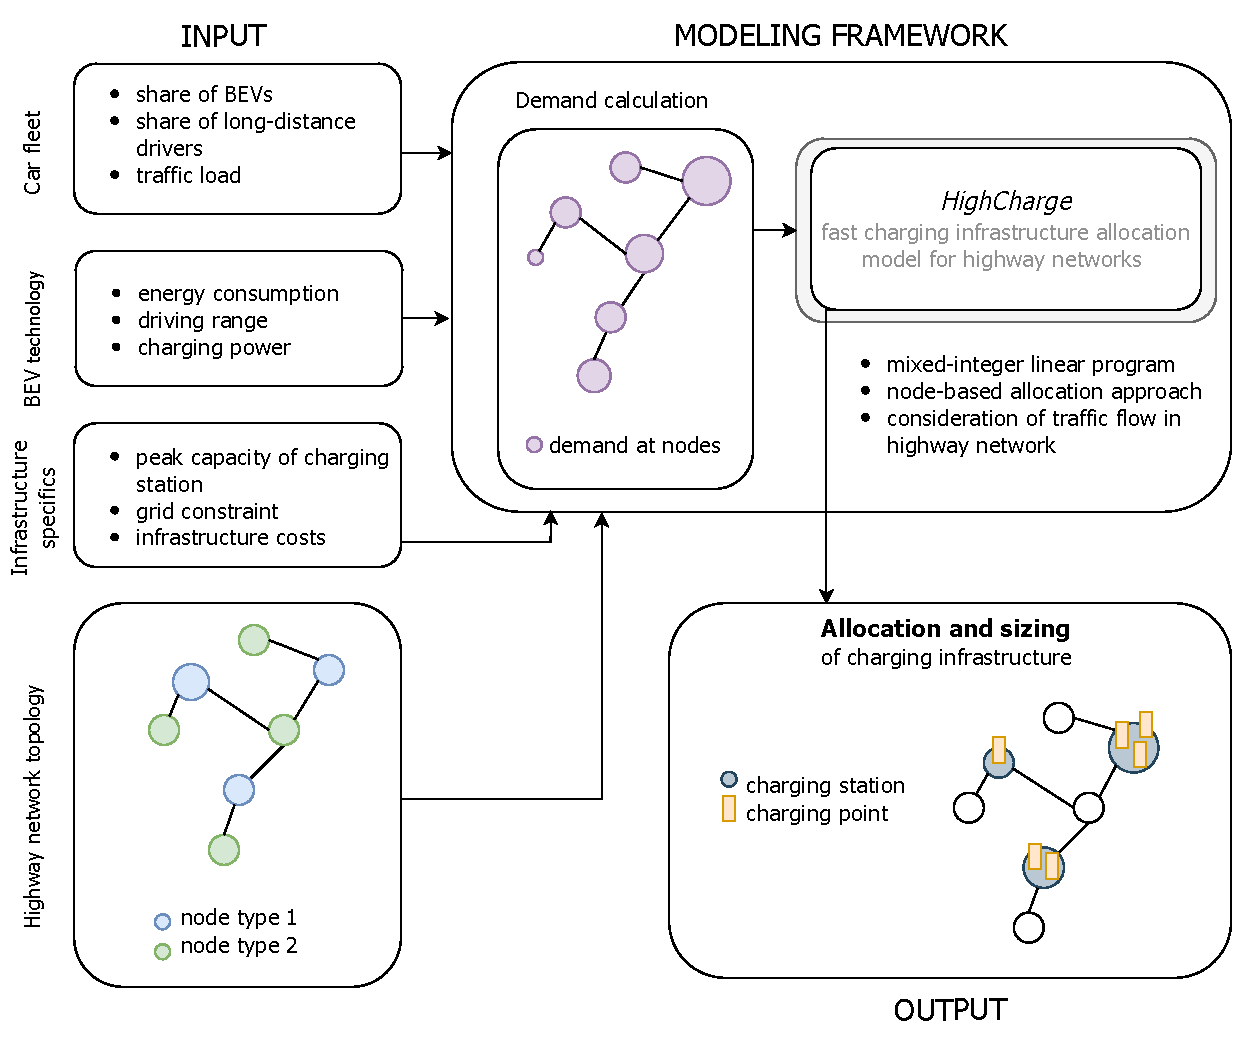
\includegraphics[width=14 cm]{images/modelling_framework.pdf}
\caption{\textbf{Overview of methodology applied in this work.} Input parameters encompass demand calculation and optimization determining the allocation and sizing of charging infrastructure.\label{fig:method}}
\end{figure}   

Before continuing with the mathematical formulation of the proposed modeling framework, we elaborate on the key assumptions underlying the methodology:  

\begin{itemize}

     \item The costs of a charging station include, on the one hand, onsite preparations to enable the support of large capacities given by the charging points locally ($c_X$) and, on the other hand, hardware and construction costs associated with the installation of one singular charging point ($c_Y$).
     
      \item Service areas along highways are potential sites for charging stations. Areas that only offer parking places are not considered as potential sites due to limited space and infrastructure on site.
     
     \item The BEV fleet traveling along the highway network is treated as a homogeneous quantity, allowing to consider accumulated charging demand and translating this into the optimal sizing of a charging station. Based on this assumption, the technical parameters of an \textit{average} BEV are assumed, such as average driving range ($\overline{dist}_{range, BEV}$), energy consumption ($\overline{d}_{spec, BEV}$) and charging capacity ($\overline{P}_{charge,BEV}$).
 
    \item All charging demands, $\sum_{n, k}\hat{D}_{n_k}$, result from the energy consumption of BEVs driving along the highway and need to be compensated for in total by charging stations built along the highway network.

    \item Highway charging infrastructure is primarily used by long-distance drivers as BEV owners mostly charge at home or at work. 

    \item A fast-charging infrastructure along a highway network is designed based on peak demands, including seasonal peak demand ($\hat{f}_{l_k}$) and hourly peak demand, during a day ($\gamma_h$).
      
   
   
    %\item Overall, the modeled charging infrastructure represents a minimum requirement to support long-distance travel with BEVs given current technological standards.  
\end{itemize}





    % Figure ... explains this calculations visually. 
    
    % two figures: applied GRNN + integral 
    
    \subsubsection{Optimization model}
    % Objective function
    The objective function of the optimization model is to minimize the total charging infrastructure investment costs: 
        
    \begin{linenomath}
        \begin{equation}
                \min_{X_{l}, Y_{l_k}, \hat{E}_{l_k}^{charged, n_k}, \hat{D}_{l_k}^{in, n_k}, \hat{D}_{l_k}^{out, n_k}}  c_{X} * \sum_{l} X_{l} + c_{Y} * \sum_{l_k} Y_{l_k}
        \end{equation}
    \end{linenomath}
    
    The charging infrastructure is designed in such a way that all demand $\sum_{n, k}\hat{D}_{n_k}$ in the network is covered. For each node the following energy balance is defined:
    
    \begin{linenomath}
        \begin{equation}
                \hat{E}_{l_k}^{charged,n_k} - \hat{D}_{l_k}^{demand,n_k} =  \hat{D}_{l_k}^{out, n_k} - \hat{D}_{l_k}^{in, n_k} \quad : \forall n_k, l_k \in A_{n_k}\\
        \end{equation}
    \end{linenomath}
    
    Set $A_{n_k}$ encompasses all nodes $l_k$ which are within the distance of $dist_{max}$\footnote{$dist_{max}=\nicefrac{4}{5} * 0.6 * \overline{d}_{range, BEV}$: The factor $\nicefrac{4}{5}$ accounts for reduced driving range resulting from increased energy demand at highway speeds \cite{Baresch2019, Napoli2020}and $0.6$ for charging processes starting at a state of charge of 20\% up to 80\% \cite{NEUBAUER201412}.} to node $n_k$. Within this set radius around a node $n_k$, the energy demand stemming from node $n_k$, $\hat{D}_{n_k}$ has to be covered. Between the nodes $l_k$, which are part of $A_{n_k}$, the demand is shifted and for this, the following holds for adjacent nodes $l_k$ and $l'_k$:
    
    \begin{linenomath}
        \begin{equation}
               \hat{D}_{l_k}^{out, n_k}  * r_{l_k, l'_k} = \hat{D}_{l'_k}^{in, n_k} \quad : \forall n_k, \{l_k, l'_k\} \in A\replaced{_{n_k}}{^{n_k}}\\
        \end{equation}
    \end{linenomath}
    
        For parameter $r_{l_k, l_k'}$, the following applies:
    
    
    \begin{linenomath}
        \begin{equation} \label{form:1}
    r_{l_k, l'_k} = 
        \begin{cases}
            1,& \text{if } s_{l_k} == s_{l_k'}\\
            <1,              & \text{otherwise}
        \end{cases}
        \end{equation}
    \end{linenomath}

    \begin{linenomath}
        \begin{equation} \label{form:2}
            \sum_{l_k} r_{l_k, l'_k} = 1
        \end{equation}
    \end{linenomath}

    This rationing parameter is, therefore, only lower than 1, if node $l$ is a junction point and in this case, the $\hat{D}_{l_k}^{output, n_k}$ needs to be split to simulate traffic flow partitioning at a junction point. For example, if, e.g., three segments meet and it is assumed that traffic flow is split equally between these segments at the junction, then $r=\nicefrac{1}{2}$.  

    
    The demand coverage by a charging point and charging station is defined through: 
    \begin{linenomath}
        \begin{equation}
               \sum_{n_k} \hat{E}_{l_k}^{charged,n_k} \leq \sum_k Y_{l_k} * \overline{P}_{charge, BEV} \quad : \forall l_k  
        \end{equation}
    \end{linenomath}
    
    
    
    \begin{linenomath}
        \begin{equation} \label{equ:max_cap}
               \frac{P_{max}}{\hat{P}_{CP}} * X_{l} \geq \sum_k Y_{l_k} \quad : \forall l 
        \end{equation}
    \end{linenomath}
    
    Equation \ref{equ:max_cap} establishes the relation between the sizing of a charging station, i.e.\added{,} the number of charging points, and the binary variable, whether a charging station is installed at node $n_k$. 
    

    
    

    \subsubsection{Charging demand calculation}
    
    To each node $n$ in the network, a charging demand is assigned for each direction $k$ from which it is accessible. For this, daily traffic counts are utilized to estimate the number of cars passing  at all node positions \replaced{$n$ and driving in direction $k$}{$n_k$}. To take into account the demand of maximum traffic load to the charging infrastructure in the analysis, the maximum daily traffic count values are obtained from the measurements performed for a span of 1 year. 
    Then, the following is performed for each segment $s$ in the direction $k$ of the highway network: All traffic counter positions lying on $s$ are mapped onto the segment, and a function expressing traffic load in dependence of the distance in the traveling direction is approximated using the general regression neural network (GRNN) model, which is able to estimate various forms of underlying functions using Gaussian functions given few input data points \citep[][]{Gholamrezaei2007}. Using the function, $GRNN_{sk} (dist)$, the peak daily traffic loads are approximated for all nodes $n$, which lie on segment $s$ and are accessible from the driving direction $k$:
    
    
    \begin{linenomath}
        \begin{equation}
            \hat{f}_{n_k}=GRNN_{s_k} (dist_{ns_k})
        \end{equation}
    \end{linenomath}
    
    To obtain the charging demand at node $n_k$ resulting from the energy consumed along the distance driven since passing the last node $n-1_k$, the integral between these distances is calculated and multiplied by the specific energy demand $\overline{d}_{spec, BEV}$ by one BEV:

    \begin{linenomath}
        \begin{equation}
            \hat{D}_{ns_k} = \overline{d}_{spec, BEV} * \epsilon * \mu * \gamma_h * \alpha \int_{dist_{n-1}}^{dist_n} GRNN_{s_k} (dist),  \mathrm{d} dist 
        \end{equation}
    \end{linenomath}
    
    $\epsilon$ describes the share of BEVs in the car fleet, whereas $\mu$ expresses the share of long-distance drivers. Factor $\gamma_h$ expresses the share of daily travels appearing during the peak hour of a day. Parameter $\alpha$ is introduced as a factor that allows to express relative changes in the overall traffic load along highways between the year during which the traffic counts were obtained and the year for which the demand is modeled; this allows to take into account the decrease in road traffic due to activity reduction or modal shift. Rationing parameter $r$ \added{(in Formulas \ref{form:1}, \ref{form:2})} is defined for each junction based on the values approximated for the given node by the function $GRNN_{sk} (dist)$ of all segments, the junction node is part of. 
    
    

    \subsection{Case study, scenarios and input data}
    
    \subsubsection{Austrian case study}
    The proposed modeling framework is applied to Austria`s highway network by modeling a cost-optimal charging infrastructure expansion for 2030 under different future scenarios. In this study, year 2030 has been chosen here mainly due to the two following reasons: first is that the aim of the analysis of this paper is to illustrate short-term infrastructure requirements (short term in terms of infrastructure planning), and second is that it is a significant year in decarbonization plans for the transport sector as the Paris Agreement explicitly states a 20\% electrification of global road transport by 2030 \citep{paris}.   
    
    To extrapolate future scenarios, model input parameters were set, which describe the current status of Austria in 2021. Table \ref{tab:val} presents the selected values. Until the end of December 2021, $76,539$ electric vehicles have been registered in Austria \citep{beoe}, which make up for 1.5 \% of all the registered passenger cars in Austria. In order to determine traffic load on highways during peak hour and the share of long-distance drivers, the most recently acquired data (Austrian-wide) on mobility patterns was used \citep{mob_survey}. Similar to the work of \citet{Jochem2016}, it was assumed that all car trips taking longer than 45 min and are longer than $25km$ or car trips longer than $50km$ are most probable to include driving on highways or motorways. Furthermore, trips were classified as long-distance if the drive was at least $100km$ long, following the common definition of \textit{long-distance} travel \citep{frei2010long}. Based on the starting times of these trips, it was evaluated that during the hour of peak demand on Austrian highways $12\%$ of the daily traffic takes place and 24\% of the traffic are long-distance travelers. 
    
    Traffic counts were obtained from \citet{asfinag}, which provide averaged weekly traffic counts for up to 276 positions along Austrian`s highways and motorways. Their data encompasses counts for vehicles of two categories, namely: vehicles weighing up to 3.5 tons and those weighing greater than 3.5 tons. As no differentiation is made between light-duty vehicles and passenger cars in the category of $< 3.5$ tons, it was assumed that all vehicles of this category are passenger cars, as light-duty transport will also be transitioned to electromobility \citep{Nachhaltig}. Data for the year 2019 was chosen to be representative for 2021 as the complete data set for 2021 has not been published as of the time of the conduction of this analysis, and the 2020 dataset cannot be used due to \added{being effected by the} month-long lockdowns during the COVID pandemic. 
    
  The technical parameters $\overline{d}_{spec, BEV}$, $\overline{dist}_{range, BEV}$, and $\overline{P}_{charge, BEV}$ were set in such a way that they would represent an average Austrian BEV. For this, the technological attributes of the respective top 10 sold cars during the years 2019, 2020 and 2021 were used to evaluate the average values (see Appendix \ref{app:param} for details on this).
    
    Infrastructure cost component $c_X$ is particularly difficult to set here as these onsite preparation costs may significantly vary based on the location of the site.
    Indications for the approximation of this value were drawn from \cite{Jochem2016}, \cite{Serradilla2017} and \cite{Verein2019}. The installation costs of one charging point, $c_Y$, was assumed to be €$60,000$ for the hardware of a charging pole with $\hat{P}_{CP} = 150kW$ --- which currently enables the fastest charging of passenger cars; an added construction costs to be €$7,000$ \citep{Verein2019, Suarez2019}. Furthermore, it was assumed that the maximum installed capacity at a charging station is $12 MW$.
    
       The shape of the Austrian highway and motorway network was mapped based on geographic data by \citet{OpenStreetMap}. The positions of the service areas were gathered based on the information drawn from \citet{asfinagrastanlagen} and complemented with geographic information from \citet{OpenStreetMap}. The retrieved highway network used throughout the analysis has an overall length of $220km$ and consists of $55$ segments. Moreover, there are $249$ nodes in total, $139$ of which represent service areas and $110$ junctions. \added{Further details on data preparation are found in the Appendix \ref{app_3}.}

    
    

        
    
    \begin{table}[h]
    \centering
    	
    \caption{Model input parameters reflecting the status quo in Austria. \label{tab:val}}
    \begin{tabularx}{\textwidth}{@{}ll@{}}
    \toprule
    
    \multicolumn{2}{l}{\textbf{Base case}}                                                                          \\ \midrule
    Input parameter & Value\\ \midrule
    BEV share $\epsilon$          &  $1.5\%$ \\
    %source: https://de.statista.com/statistik/daten/studie/688862/umfrage/anteil-der-elektro-pkw-in-oesterreich/)  \\
    Share of traffic load during peak hour $\gamma_h$ &  $12\%$ \\
    Share of long-distance drivers $\mu$ & $24\%$  \\
    

                               
    \begin{tabular}[l]{@{}l@{}}Share of overall traffic load compared with \\ the survey year of traffic counts  $\alpha$ \end{tabular}         & $100\%$    \\
    traffic count data $\hat{f}_{ik}$ & maximum \added{recorded} daily traffic counts 2019
    \\
    \begin{tabular}[l]{@{}l@{}}energy consumption of an average BEV \\ in the car fleet $\overline{d}_{spec, BEV}$  \end{tabular}              & $0.24 kWh/km$  \\
    
    \begin{tabular}[l]{@{}l@{}}driving range of an average BEV \\ in the car fleet $\overline{dist}_{range, BEV}$  \end{tabular} &  $340km$\\
    
    \begin{tabular}[l]{@{}l@{}} charging capacity of an \\ average BEV $\overline{P}_{charge, BEV}$  \end{tabular}  & $81 kW$ \\
    peak capacity of a charging point $\hat{P}_{CP}$  & $150 kW$\\
    \begin{tabular}[l]{@{}l@{}} maximum installed charging capacity \\ at a charging station $P_{max}$ \end{tabular} &  $12 MW$\\
    
    
     \begin{tabular}[l]{@{}l@{}}investment costs for installation \\ a charging station $c_{X}$   \end{tabular}             &  € $40,000$                                  \\
    %$c_{Y, 50kW}$ (€)           & 17750                                     \\
    \begin{tabular}[l]{@{}l@{}} investment costs for installation of  \\ one charging point $c_{Y, 150kW}$    \end{tabular}          & € $67,000$                                     \\

    
    \bottomrule
    \end{tabularx}%
    \end{table}
 
    \subsubsection{Future scenarios}
    Four quantitative scenarios for Austrian highway charging infrastructure expansion are outlined. These were developed in the course of the Horizon 2020 research project openEntrance \citep[][]{openentrance}. The scenarios outline pathways to climate change mitigation by reaching the $1.5^{\circ}C$ or $2.0^{\circ}C$ targets and are referred to as the \textit{Societal Commitment} (\textit{SC}), \textit{Techno-Friendly} (\textit{TF}), \textit{Directed Transition} (\textit{DT}) and \textit{Gradual Development} (\textit{GD}) scenarios. The former three pathways aim to mitigate climate change by keeping the temperature rise to a maximum of $1.5^{\circ}C$ as specified in the Paris Agreement, the latter to $2.0^{\circ}C$. Within these scenarios, the extent of societal engagement, implementations of technological novelties and the strong presence of political interventions in climate change mitigation vary \citep[see also][]{Auer2019, HAINSCH2022122067}. These scenarios were developed to outline mitigation paths for different economic sectors in Europe and are used here to align the analysis described in this paper into the large-scale context of decarbonization. Based on this, different developments of the transport sector relevant to the present work are projected:
    \begin{itemize}
        \item \textbf{Societal Commitment (\textit{SC}):} Within this scenario, politics are strongly intervening  which is met by wide-spread societal acceptance, triggering behavioral changes in the face of awareness of the necessity of climate change mitigation. While this scenario is characterized by a reduction in energy demand due to behavioral changes, societal engagement supporting circular economy, and new market solutions, it is assumed that no significant technological breakthroughs appear. This translates in the transport sector to an increased modal shift to sharing concepts and public transport, which causes a significant decrease in individual passenger road transport.
        \item \textbf{Techno-Friendly (\textit{TF}):} This setting combines the appearance of major technological breakthroughs and strong societal engagement, which results in an increased top down push effect in the application of new technologies that improve energy efficiency. Simultaneously, similarly as in the SC scenario, there is a strong social commitment driving an increased modal shift away from individual passenger car transport. 
        \item \textbf{Directed Transition (\textit{DT}):} Similarly as in the TF scenario, there is a strong active policy push  supporting new technology options. While there are major technological developments, the social commitment to adopting such developments is missing. This results in the moderate growth of BEV share throughout the years and a decreased modal shift, but registered BEVs of the Austrian car fleet still show similar technological improvements as in the TF scenario.
        \item \textbf{Gradual Development (\textit{GD}):} This scenario represents the projection of less ambitious climate change mitigation goals. It embodies the exertion of all three dimensions, namely, social engagement, technological breakthroughs, and significant political interventions, only a weaker extent of each. Therefore, while BEV penetration will grow to some degree, and technological improvements will appear, no changes in mobility patterns are expected for this pathway.  
    \end{itemize}
    

    
    Based on these scenario descriptions, we embed projections on changes in the modal split and developments in the BEV technology in European climate mitigation pathways for 2030.
    Parameters $\epsilon$ and $\alpha$ are specified based on the climate change mitigation goals for Austria`s passenger transport sector described in the governmental document \enquote{Austria's Mobility Master Plan 2030} (\texit{AMMP}) \citep{Nachhaltig}. One of these key goals is to reduce motorized private transport by $31\%$ between the years 2018 and 2040 to meet the $1.5^\circ C$ target set by the Paris Agreement. In the SC scenario where strong societal and political engagement act together, this goal will be met by 2030. The AMMP further specifies that by 2030, $100\%$ of newly registered passenger vehicles must be exclusively powered by an electric engine. In the SC and TF scenarios, it is assumed that the share of new registrations of electric vehicles will gradually increase until 100\% in 2030 due to the strong awareness of the necessity of electromobility by the society. For the \texit{DT} and \texit{GD} scenarios, the steady growth rate as experienced in 2020-2021 is projected until 2030, which will result in an EV share of $27\%$\footnote{This was calculated under the assumption that the size of the Austrian car fleet will not grow further from today.}.
    
    Table \ref{tab:technolog_params_future} presents the projected values. The presence of major technological breakthroughs is expressed by a significant development in the driving range of BEVs and increasing charging power, which is in line with the current major focus in BEV technology research on battery technology with the goal of allowing faster charging and longer trips \citep[][]{IRENA2019, Thielmann2020}. According \added{to} the study by \citet{Thielmann2020}, there is a great potential in battery storage research suggesting that technological breakthroughs in the next years could lead to the sale of BEVs with a driving range of up to $1000km$.  Based on this, the sale of BEVs with an average driving range of up to $800km$ is projected for 2030 in the TF and DT scenarios, whereas in the SC scenario, this range is assumed to be $450km$, being slightly larger than the ranges of BEVs currently on the market (see Table \ref{tab:top10} in Appendix \ref{app:param}). To reflect a weak extent of technical developments in the GD scenario, the increase in the average driving range of up to $600km$ is projected for 2030.
    
    To compare the results of the scenarios, a similar peak power for charging points is assumed for all four scenarios. The study by \citet{IRENA2019} projected $\hat{P}_{CP} = 350kW $ to be the predominant peak charging power by 2030. The costs for the hardware of a charging pole are estimated to be €120,000, as well as an additional construction cost of €7,000 \citep{Suomalainen2019, Baumgarte2021}. To reflect different improvements in charging efficiency, technological breakthroughs are assumed to lead to charging power levels of up to $\overline{P}_{charge, BEV} = 315kW$, given that the efficiency will increase up to $90 \%$, as for charging poles with peak capacity of $50kW$ nowadays \citep{Genovese2015}. Today, one of the passenger car models with the highest charging power is Porsche Taycan with $\overline{P}_{charge, BEV} = 197 kW$. For the SC and GD scenarios, this is assumed to be adopted by all BEV vehicles in 2030.  
    
    Other model input parameters are assumed to be similar as in 2021, using the values from Table \ref{tab:val}. Table \ref{tab:scenario_params} summarizes the overall projected values describing the average Austrian car fleet in 2030 which were extrapolated based on the assumption that these parameters would gradually change in a linear way until 2030 on the basis of the values for 2021 (see also Appendix \ref{app_2}). 
    

    \begin{table}[H]
    \centering
    \caption{Car fleet parameters and average technical parameters of an average BEV on the market in 2030 for different scenarios (BEV share $\epsilon$, share in road traffic $\alpha$, average driving range $\overline{dist}_{range, BEV}$, average charging power $\overline{P}_{charge, BEV}$).\label{tab:technolog_params_future}}
    \newcolumntype{C}{>{\centering\arraybackslash}X}
    
    \begin{tabularx}{\textwidth}{lCCCC}
    \toprule
                                     & \multicolumn{4}{c}{\textbf{Projections for 2030 under different scenarios}}                                                                                                                                                                                                                                \\ \cmidrule(l){2-5} 
                                Model parameters      & \textit{\begin{tabular}[c]{@{}c@{}}
                        Social \\ Commitment\end{tabular}} & \textit{\begin{tabular}[c]{@{}c@{}}Techno-\\ Friendly\end{tabular}} & \textit{\begin{tabular}[c]{@{}c@{}}Directed \\ Transition\end{tabular}} & \textit{\begin{tabular}[c]{@{}c@{}}Gradual \\ Development\end{tabular} }\\ \midrule
                                          $\epsilon (\%)$                      & 33                                                                   & 33                     & 27                                                                    & \multicolumn{1}{c}{27}                                                 \\
    $\alpha (\%)$                         & 69                                                                    & 83                     & 83                                                                    & \multicolumn{1}{c}{100}                                                                                                       \\
    $\overline{dist}_{range, BEV} (km)$          & 450                                                          & 800                                                       & 600                                                           & 800                                                             \\
    $\overline{P}_{charge, BEV} (kW)$ & 200                                                          & 315                                                        & 315                                                            & 200                                                             \\ \bottomrule
    \end{tabularx}
    \end{table}
    
 
    \begin{table}[H]
    \caption{Model parameter values projected for the scenarios of climate change mitigation, set for year 2030 (BEV share $\epsilon$, share in road traffic $\alpha$, average driving range $\overline{dist}_{range, BEV}$, average charging power $\overline{P}_{charge, BEV}$, peak charging power of a charging point $\hat{P}_{CP}$, costs of installment of one charging point $c_{Y}$). \label{tab:scenario_params}}
    
    \begin{tabularx}{\textwidth}{lCCCC}
    \toprule
                                & \multicolumn{4}{c}{\textbf{Input parameters for scenarios 2030}}                                                                                                                                                                                                                          &                                                                  \\ \cmidrule(lr){2-5}
    Model parameters            & \textit{\begin{tabular}[c]{@{}c@{}}Societal \\ Commitment\end{tabular}} & \textit{Techno-Friendly} & \textit{\begin{tabular}[c]{@{}c@{}}Directed \\ Transition\end{tabular}} & \textit{\begin{tabular}[c]{@{}c@{}}Gradual \\ Development\end{tabular}}  \\ \midrule
    $\epsilon$ $(\%)$                      & 33                                                                    & 33                     & 27                                                                    & \multicolumn{1}{c}{27}                                               \\
    $\alpha$ $(\%)$                         & 69                                                                    & 83                     & 83                                                                    & \multicolumn{1}{c}{100}                                                                                                          \\
    
    
    $\overline{dist}_{range, BEV}$ $(km)$    & 420                                                                     & 670                      & 660                                                                    & \multicolumn{1}{c}{520}                                                                         \\ 
    $\overline{P}_{charge, BEV} (kW)$    & 166                                                                    & 248                      & 243                                                                    & \multicolumn{1}{c}{164}                                                                                                  \\
    $\hat{P}_{CP} (kW)$  & 350 & 350 & 350 & \multicolumn{1}{c}{350} \\
        $c_{Y, 350kW}$ (€)    & 127,000                                                                     & 127,000                      & 127,000                                                                    & \multicolumn{1}{c}{127,000}                                                                                                        \\ \bottomrule
    \end{tabularx}%
    
    \end{table}
    

    \subsection{Model validation and limitations \label{sec:val}}
    The model is validated by modeling present day infrastructure requirements and comparing the results with \replaced{the setup}{those} of the existing infrastructure. The current infrastructure requirements are modeled using input parameters displayed in Table \ref{tab:val}. In Figure \ref{fig:comp}, the capacities of the currently installed fast-charging infrastructure along Austria´s highways (as of December 2021) are illustrated along with a comparison to the model output. Table \ref{tab:validation} presents the numbers of fast-charging points of different peak power levels and total capacity. 


    
    
    \begin{table}[h]
    \centering
    \caption{Comparison of existing fast infrastructure along Austrian highway network (as of December 2021) and model output based on the number of charging stations and summed peak power levels ($\hat{P}_{CP}$).\label{tab:validation}}
    
    \begin{tabularx}{\textwidth}{@{}lcc@{}}
    \toprule
                                                  & Existing infrastructure & Model output \\ \midrule
    Nb. charging stations                   & 31                      & 43           \\
    Nb. charging points with $\hat{P}_{CP} = 44 kW$ (AC)& 8 &  - \\
    Nb. charging points with $\hat{P}_{CP} = 50 kW$  (DC)&     72                    & -            \\
    Nb. charging points with $\hat{P}_{CP} = 75 kW$  (DC)&      4                   & -            \\
    Nb. charging points with $\hat{P}_{CP} = 150 kW$ (DC)&        22                 & 98         \\
    Nb. charging points with $\hat{P}_{CP} = 350 kW$ (DC) &         40                & -            \\ \midrule
    Total capacity (MW) & 20.1 & 14.7\\
    \bottomrule
    \end{tabularx}
    
    \end{table}
    
    

    \begin{figure}[h]
    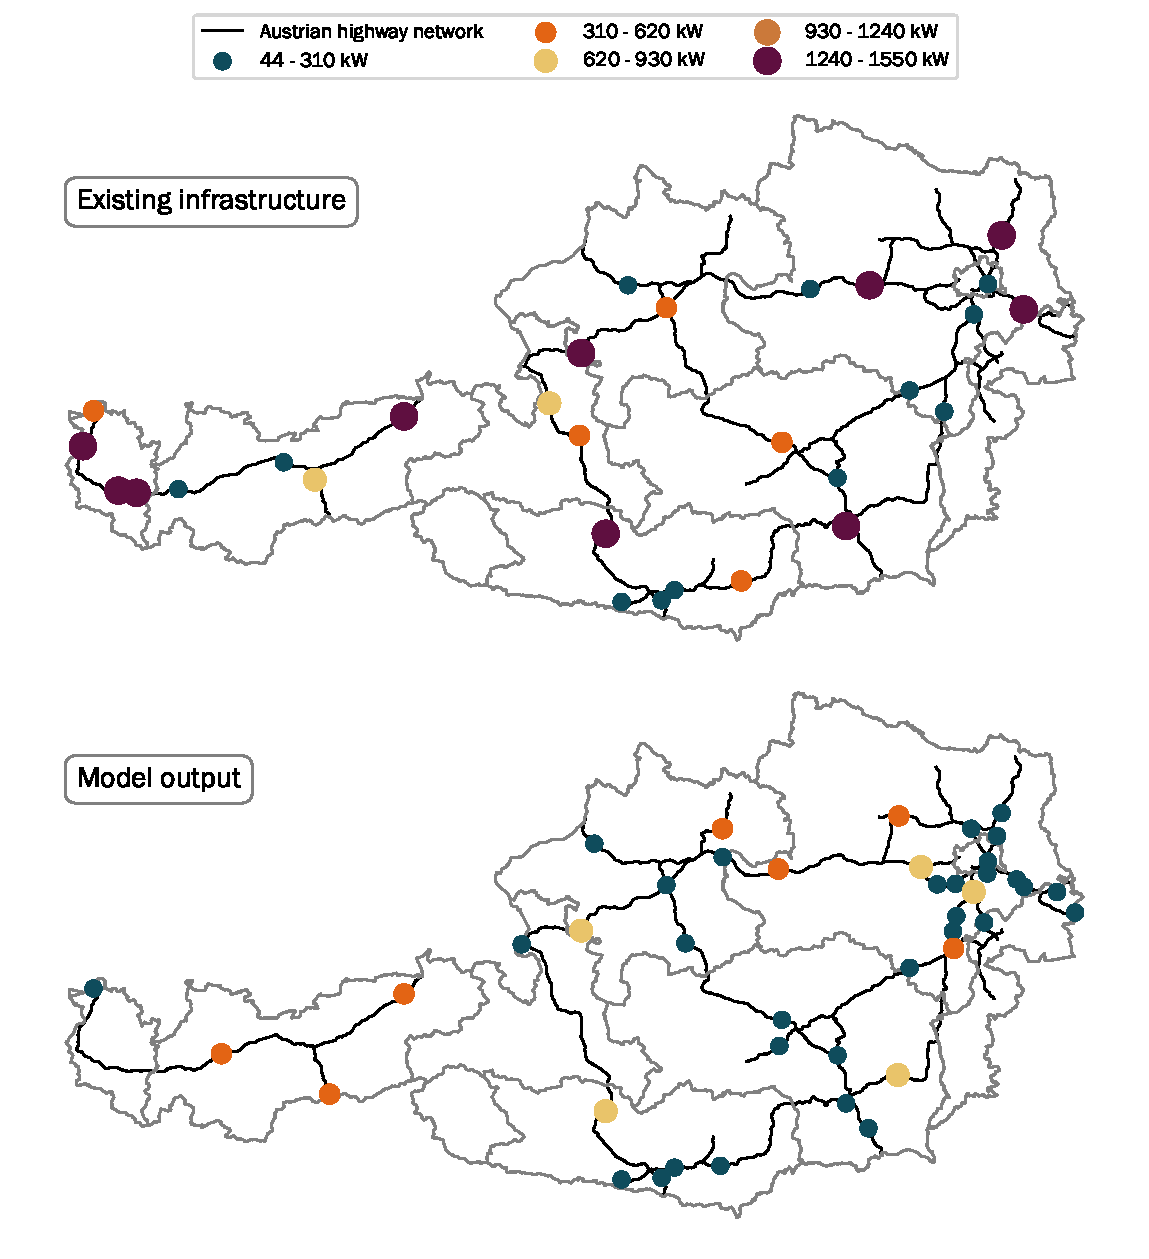
\includegraphics[width=14 cm]{images/comparison_image.pdf}
    \caption{\textbf{Model validation.} Visual comparison of the capacities, i.e.\added{,} summed peak power of all onsite charging points, in existing fast-charging infrastructure (\textbf{top}) and the modeled infrastructure (\textbf{bottom}) using on the values displayed in Table \ref{tab:val}. \label{fig:comp}}
    \end{figure}   
    \unskip
    
   

    While the overall amount of the charging stations seems to be in a similar range, a gap appears to exist between the total installed capacity estimated by the model versus the existing capacity. There are several possible reasons for this. One might be that the proposed modeling framework aims to design a minimum required charging infrastructure for a given point in time, therefore, no pre-planned charging capacities with regard to developments in the future is modeled. In existing infrastructure, this is not the case as, for example, IONITY \citep{ionity}, the joined venture by multiple cars producers, has installed most of the charging points with $\hat{P}_{CP}=350kW$ while currently only few cars on the market are able to charge at a power level above $150kW$ \citep{Suarez2019}. Therefore, in this context, the modeled infrastructure reflects the minimum requirements for a fast-charging infrastructure. Moreover, the difference could stem from the fact that the model assumes charging points of a singular peak power level and all BEVs of the Austrian car fleet having the same technical parameters which makes it difficult to directly compare existing and modeled capacity because the charging points of different peak power levels have different efficiencies and the average charging capacity varies significantly among car models \citep[see e.g.][]{Suarez2019}. 
    
    The difference in the location distribution of capacities can be attributed to the model assumption that the proportion of long-distance travelers among highway traffic is equal throughout the whole highway network. Further, local differences of the cost parameter $c_X$ are neglected, whereas in reality, this cost component significantly varies depending on the location \citep{Serradilla2017}. Another reason for the difference in site allocation can be that within the model, all energy is aimed to be covered and given the geographical boundary of Austria, charging stations lying right outside the countries boarders are not considered. Therefore, the model tends to install charging stations at service areas that are closest to the end points of the highway network to cover all demands within the network. Another striking difference between existing and modeled fast-charging infrastructure is the accumulation of many small charging stations in the vicinity of Vienna, which lies in the East of Austria, in the modeled infrastructure. Some of them may stem from the tendency of installing charging infrastructure near borders, whereas others are most likely installed there due to the dense topology of the highway network around Vienna. \citet{Jochem2019}, who modeled fast-charging infrastructure along the European highway network, also observed that within networks of higher densities, more and smaller charging stations are \replaced{placed by the allocation model}{modeled}.   
    
    
    \subsection{Open-source programming environment and data availability}
    
    The described modeling framework was implemented using Python 3.8 and the Python package \textit{pyomo} 6.2 \cite{hart2011pyomo}. All materials for the analysis in this paper are publicly available on GitHub\footnote{\url{https://github.com/antoniagolab/HighCharge})}. In the application of the mixed-integer linear program in the Austrian case study, the number of nodes is 249. The number of constraints is about 1.3 Mio. and varies slightly depending on the input parameter expressing the average driving range of BEVs, $\overline{dist}_{range, BEV}$. The time of a model run heavily depends on the specified BEV driving range: For example, at $400km$, the total model run takes $650 s$, and at $800km$, $1360 s$, yielding a solution of up to an optimality gap of 0.2\%. 
 
%%%%%%%%%%%%%%%%%%%%%%%%%%%%%%%%%%%%%%%%%%

\section{Results}
In this section, the most relevant results are presented. It is divided into two parts: First, we elaborate on the expansion requirements for the existing fast-charging infrastructure along Austria's highway network under different future scenarios for 2030. Details on the results obtained for the DT scenario, for which the costs of fast-charging infrastructure expansion are the lowest, are presented. Subsequently, the results of the modeled expansion given four different scenarios, SC, TF, DT and GD, are compared based on parameters describing the costs and the required charging infrastructure expansion. To gain better insight into how the observed differences between the scenarios come to place, \deleted{the} selected input parameters of the scenario result with the highest infrastructure expansion costs for 2030, which is the GD scenario, are altered. In the second part of this section, the focus shifts from the required infrastructure expansion for 2030 to the analysis of changing infrastructure requirements in the face of technological development and increasing demand. First, the effect of change in the driving range of an average BEV is observed and, second, that of increasing demand by the rising share of BEVs in the Austrian car fleet. 


\subsection{Expansion of fast-charging infrastructure along Austrian highway network under different scenarios for 2030}

Under the consideration of existing charging points with the peak capacity of $\hat{P}_{CP} = 350kW$, which is assumed to be the predominant charging capacity of fast-charging infrastructure for 2030, and the assumption that the investment of on-site preparation ($c_X$) has been made for all existing charging stations with charging points allowing fast-charging, the expansion of the current charging infrastructure along the Austrian highway network was modeled under different climate mitigation scenarios. 

\subsubsection{Austria`s fast-charging infrastructure for 2030 under the Directed Transition scenario}


Table \ref{tab:spec_res} and Figure \ref{fig:expansion_dt_2030} display the modeling results for the expansion of the current $350kW$ charging infrastructure along highways in Austria for 2030 under the DT scenario. In Figure \ref{fig:expansion_dt_2030}, the charging infrastructure expansion is expressed through additionally needed capacities. The expansions at existing charging points are indicated in dark \replaced{green}{blue and green}, and required capacities at newly installed charging points are indicated in orange \deleted{and red}. The charging stations in \replaced{the lighter shades of green and orange}{turquoise and orange} indicate the required expansion of $350 - 4900 kW$, i.e., by 1-14 charging points, and charging stations in \replaced{the darker shades}{dark blue and red} installations of additional $5200 - 10500 kW$, i.e., 15 - 28 additional charging points. The total infrastructure expansion costs are estimated to be €54 Mio., which are translated to €/kW 369 and €39 per registered BEV in the Austrian car fleet in 2030. While currently, 40 charging points with $\hat{P}_{CP}=350 kW$, i.e., $14 MW$, are \deleted{currently} installed along Austrian highways, an additional $+146 MW$ of charging capacity are required until 2030. Further, additional $24$ charging stations are needed, of which 10 are positioned within the dense part of the highway network in the East of Austria, in the vicinity of Vienna. The results also indicate\deleted{d} the need for the installation of new charging stations near the Austrian border in order to cover all demand within the boarders, which mostly results from the model formulation enforcing all coverage of demand within the network as described in Section \ref{sec:val}. Aside from this, there exist three charging stations that do not need any infrastructure expansion.

% The modeled expansion of the charging infrastructure covers up to 94.6 \% of the total energy demand along the highway network. The 5.4\% of not covered energy demand corresponds to the demand with results from the energy consumption by vehicles driving between a service area near the ending node to the ending point of the highway network. This cannot be covered within the network as no charging points can be built at network ends but only at service areas.
%Figure \ref{fig:expansion_dt_2030} displays the specific positions of required infrastructure expansion and further how much of capacity expansion is needed at existing charging points versus the amount and capacity of newly planted charging points which is overall 

    \begin{table}[h]
    \centering
    % \begin{adjustwidth}{-\extralength}{0cm}
    \caption{Cost parameters and charging infrastructure attributes resulting from the expansion of the existing $\hat{P}_{CP}=350kW$ charging infrastructure under the \textit{Directed Transition} (\textit{DT}) scenario. \label{tab:spec_res}}
    \newcolumntype{C}{>{\centering\arraybackslash}X}
    \begin{tabularx}{\textwidth}{@{}lcccccc@{}}
    \toprule
            & \begin{tabular}[c]{@{}c@{}}Nb. of charging\\  stations\end{tabular} & \begin{tabular}[c]{@{}c@{}}Total\\ capacity\end{tabular} & \begin{tabular}[c]{@{}c@{}}Specific \\capacity costs\end{tabular} & 
            \begin{tabular}[c]{@{}c@{}}Specific costs \\ per BEV \end{tabular} & \begin{tabular}[c]{@{}c@{}} Total expansion \\ costs\end{tabular} \\ \midrule
DT scenario 2030 &     54  &              $160 MW$                                                  &    €/kW 369    &            €/BEV 39                                                                                                                        &                       € 54 Mio.                                                      \\ \bottomrule

    \end{tabularx}
    % \end{adjustwidth}
    \end{table}
    

    \begin{figure}[]
    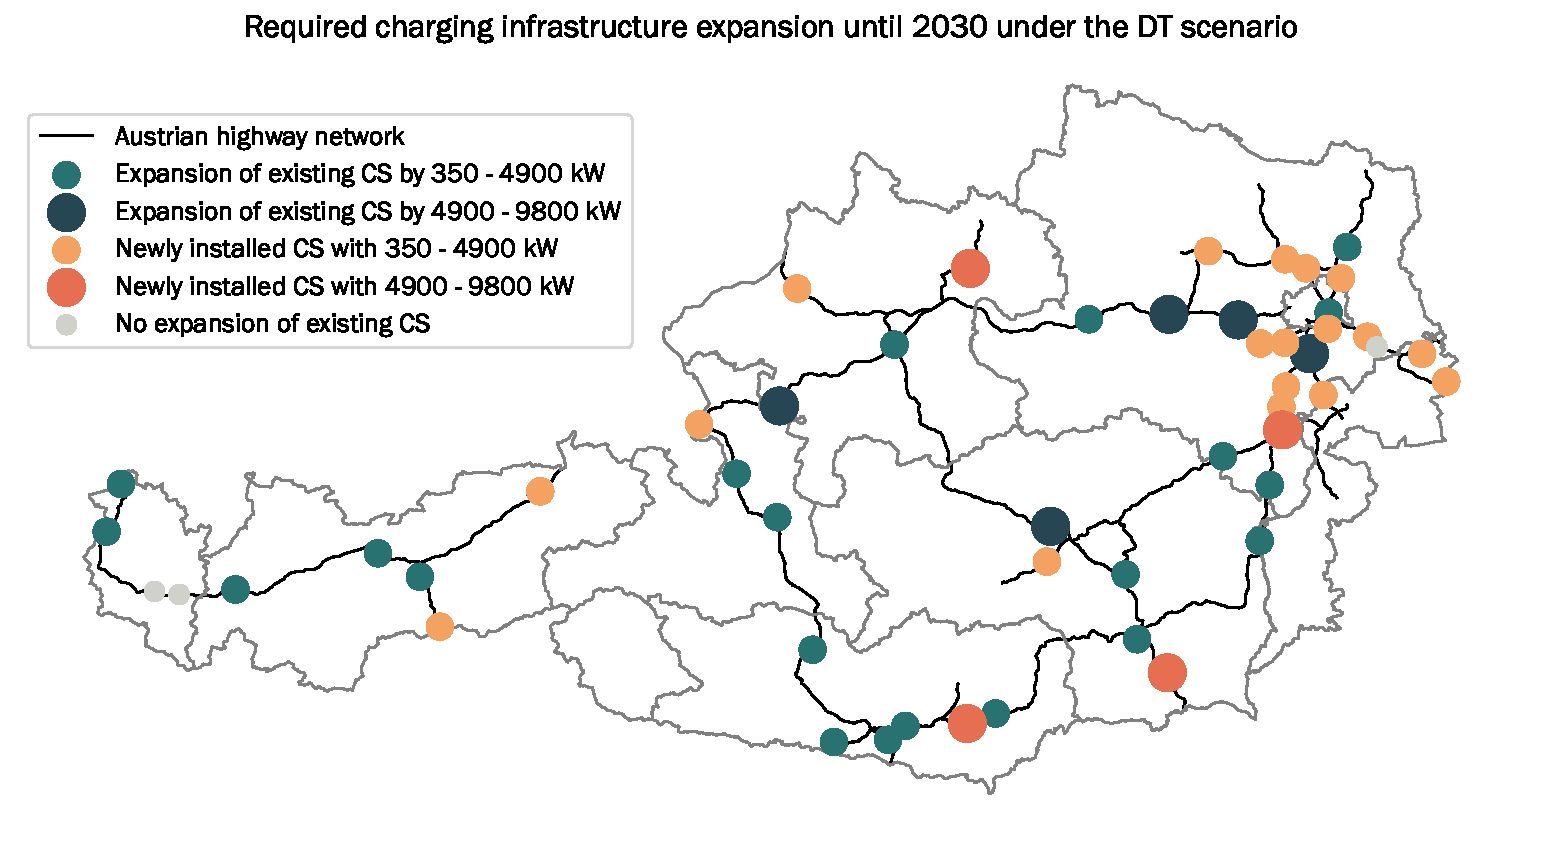
\includegraphics[width=14 cm]{images/expansion_image.pdf}
    \caption{\textbf{Required expansion of fast-charging infrastructure along Austrian highways in 2030.} Sizing of capacities that need to be added at currently existing and nonexisting charging stations (\textit{CS}) given the \textit{Directed Transition} (\textit{DT}) scenario. \label{fig:expansion_dt_2030}}
    \end{figure}   
    \unskip

% \begin{itemize}
%     \item The results suggest a required expansion of $+...\%$ of charging capacities, compared to currently existing $350 kW$ - charging infrastructure. Further, the results hint at the requirement of new charging points in the area around Vienna. 
%     \item The expansion costs are estimated to be $\EUR{blabla} Mio.$, resulting in specific costs of $\EUR{blabla}/ $ which also translates to $\EUR{blabla}/ $ per BEV. 
%     \item Densification by at least + 24 additional charging stations 
% \end{itemize}

\subsubsection{Comparison of the results  from different future scenarios}



Table \ref{tab:scenario_res} presents a comparison of key parameters describing the required infrastructure expansion under different future scenarios for Austria in 2030. The following observations are made:
\begin{itemize}
    \item The expansion under the DT scenario ,for which the input parameters were set based on the assumption of a strong presence of political incentives pushing technological developments, results in the lowest costs of charging infrastructure expansion (€54 Mio.). 
    
    \item There is a relative difference of up to $+84\%$ between the scenario causing the minimum expansion costs (DT) and the highest costs arising in the GD scenario, within which weaker climate change mitigation measures are assumed.
    
    \item The number of charging stations remains in a similar range for all scenarios, varying between 54 and 57. The specific infrastructure expansion costs per $kW$ remain also very stable at around €/kW 368.
    
    \item The specific costs per BEV range between 39 and 72 and are the lowest in the TF and DT scenarios. The common trait of these two scenarios is the presence of technological breakthroughs leading to higher driving ranges and charging capacity of BEVs. 
\end{itemize}



\begin{table}[H]
\caption{Comparison of the results for expansion of fast-charging infrastructure expansion along Austrian highways under different scenarios for 2030. The lowest specific costs per BEV and lowest total infrastructure expansion costs are highlighted. \label{tab:scenario_res}}
\resizebox{\textwidth}{!}{%
\begin{tabular}{@{}lcccc@{}}
\toprule
                            & \multicolumn{4}{c}{Scenarios 2030}                                                           &                                                                  \\ \cmidrule(lr){2-5}
Model output            & \textit{\begin{tabular}[c]{@{}c@{}}Societal \\ Commitment\end{tabular}} & \textit{Techno-Friendly} & \textit{\begin{tabular}[c]{@{}c@{}}Directed \\ Transition\end{tabular}} & \textit{\begin{tabular}[c]{@{}c@{}}Gradual \\ Development\end{tabular}} \\ \midrule
% infr costs als letztes 
% am Ende machts mehr Sinn, sonst kann man damit nichts anfangen

Nb. charging stations                     &                                                            \replaced{54}{57}       &          \replaced{53}{55}          &             54                                                        & 56                                                 \\
Total capacity (MW)                      &     238                                                              &       192            &             160                                                        & 285                                               \\
Specific capacity costs (€/kW)                       &    368                                               & 368                 &               369       &     367                                                                                                                                                           \\ 
Specific costs per BEV (€/BEV) & 49 & \cellcolor[HTML]{e5e5e5} 39 & \cellcolor[HTML]{e5e5e5}  39 &  72                                                                          \\ 
Total infrastructure expansion costs (€)                    &               8\replaced{5}{2} Mio.                                                    &          6\replaced{8}{6} Mio.         &     \cellcolor[HTML]{e5e5e5} 54 Mio.                                                              & 100 Mio.                                                \\

 \midrule
Rel. change of costs to  DT scenario                      &   $+$\replaced{57}{51}\%                                             & $+$\replaced{26}{22}\%                  &              -      &    $+85\%$                                                               \\ 

% hier in "Mio" ausdrücken !! 
% nur max. 1 Nachkommast. 
% add rel. changes to minimum solution; weniger abs Zahlen 
% average distance between charging stations (km)   &                                                                      &                       &                                                                      & \multicolumn{1}{c}{}                                                                                                            \\
\bottomrule
\end{tabular}%
}
\end{table}

% While infrastructure installment costs for the \textit{SC}, \textit{TF} and \textit{GD} scenarios are in similar range, the costs of the \textit{DT} significantly smaller compared then in the others. The \textit{DT} scenario is characterized by strong policy incentives triggering significant technological developments and a weak societal participation in achieving $1.5 \circ C$ climate targets. This results in fewer but simultaneously also in technologically further developed BEVs in the Austrian car fleet. As overall, the number of  charging points is in similar range for all scenarios, he vastly fewer infrastructure costs may stem from the smaller amount of required capacity expansion which are, on the one hand, tightly related to the smaller share of BEVs ($\epsilon$), and, on the other hand, might be due to the higher average charging capacity of BEVs ($\overline{P}_{average, BEV}$).

% \begin{itemize}
%     \item High sensitivity to the given parameters
%     \item high uncertainties in charging infrastructure planning
%     \item 
% \end{itemize}




\subsubsection{Cost-reduction potentials in the Gradual Development scenario} \label{sub:res_costred}

To shed light into why the infrastructure expansion costs in the GD scenario are up to \replaced{$+85\%$}{$+84\%$} higher than in the other scenarios and how the high specific costs per BEV of €/BEV 72 come to place, \deleted{the} selected input parameters are altered and the effects on the costs are observed. These alterations reflect developments which are absent in the GD scenario but present in the others and which essentially lead to a cost reduction in charging infrastructure expansion investments. The following projections are drawn from the other scenarios and based on these, input parameters are altered in the GD scenario: a medium decrease in road traffic by $-17\%$ until 2030 as in the TF and DT scenarios, a major decrease by $-31\%$ as in the SC scenario, technological breakthroughs as in the TF and DT scenarios altering the driving range of an average BEV sold in 2030 to be $800km$, and having an average charging capacity of $315kW$ at a charging point with $\overline{P}_{CP} = 350 kW$. Further details on these alterations are displayed in Table \ref{tab:cost_red}. 

Figure \ref{fig:cost_red} and Table \ref{tab:cost_red_2} display the resulting cost reductions and changes in the required fast-charging infrastructure in response to the respective parameter changes. The lowest infrastructure expansion costs are achieved through the increase of BEV charging power which causes a large decrease in the required capacity as the efficiency of charging increases. Similarly, high cost reduction is accomplished \deleted{through} by decreasing the overall traffic load which essentially reduces the demand for charging infrastructure. No cost reduction results from the increase in BEV driving range. Figure \ref{fig:cost_red} illustrates these changes in costs in response to the specific parameter alterations visually. 
% Please add the following required packages to your document preamble:
% \usepackage{booktabs}
\begin{table}[H]
\centering
\caption{Description of input parameter alterations reducing costs in the \textit{Gradual Development} (\textit{GD}) scenario. The parameter alterations are based on the other three scenarios: \textit{Societal Commitment} (\textit{SC}), \textit{Techno-Friendly} (\textit{TF}),  \textit{Directed Transition} (\textit{DT}). \label{tab:cost_red}}

\begin{adjustwidth}{-\extralength}{0cm}
\begin{tabularx}{\fulllength}{@{}llccc@{}}
\toprule
\textbf{Parameter change}       & \textbf{Description (reference scenario)}                                                                                                      & \textbf{\begin{tabular}[c]{@{}c@{}}Altered input \\ parameter\end{tabular}} & \textbf{\begin{tabular}[c]{@{}c@{}}Value in \\ GD scenario\end{tabular}} & \multicolumn{1}{l}{\textbf{Updated value}} \\ \midrule
Medium decrease in road traffic & \begin{tabular}[c]{@{}l@{}}The overall road traffic load is subject \\ to a reduction of $-17\%$ (DT, TF).\end{tabular}            & $\alpha$                                                                    & $100\%$                                                                  & 83 \%                                      \\
Major decrease in road traffic  & \begin{tabular}[c]{@{}l@{}}The overall road traffic load is subject \\ to a reduction of $-31\%$ (SC).\end{tabular}            & $\alpha$                                                                    & $100 \%$                                                                 & $69\%$                                     \\
Increase in driving range       & \begin{tabular}[c]{@{}l@{}}The driving range of BEVs being sold \\ in 2030 is increased to $1000km$ (DT, TF).\end{tabular}         & $\overline{dist}_{range, BEV}$                                                         & $520km$                                                                  & $660km$                                    \\
Increase in charging power   & \begin{tabular}[c]{@{}l@{}}The average charging capacity of BEVs \\ sold in 2030 is projected to be $315kW$ (DT, TF).\end{tabular} & $\overline{P}_{charge, BEV}$                                                & $164kW$                                                                  & $243kW$                                    \\ \bottomrule
\end{tabularx}
\end{adjustwidth}
\end{table}

\begin{table}[H]
\centering
\caption{Changes in fast-charging infrastructure and associated investment costs in the face of different cost-reduction measures as described in Table \ref{tab:cost_red}. The highest cost reductions are highlighted. \label{tab:cost_red_2}}
\begin{adjustwidth}{-\extralength}{0cm}

\begin{tabularx}{\fulllength}{lccccc}
\toprule
                                                    & \multicolumn{1}{l}{\textbf{}} & \multicolumn{4}{c}{\textbf{Cost-reduction measures}}                                                                                                                                                                                                                                                 \\ \cmidrule(l){3-6} 
                                                    & GD scenario 2030              & \begin{tabular}[c]{@{}c@{}}Medium decrease\\ in road traffic\end{tabular} & \begin{tabular}[c]{@{}c@{}}Major decrease\\ in road traffic\end{tabular} & \begin{tabular}[c]{@{}c@{}}Increase in\\ driving range\end{tabular} & \begin{tabular}[c]{@{}c@{}}Increase in\\ charging power\end{tabular} \\ \midrule
Nb. of charging stations                              & 54                            & 54                                                                        & 54                                                                       & 55                                                                  & 54                                                                      \\
Total capacity $(MW)$                           & 285                           & 238                                                                       & 197                                                                      & 286                                                                 & 139                                                                     \\
Total expansion costs (€) & 100 Mio.                       & 82 Mio.                                                                   & 68 Mio.                                                                  & 100 Mio.                                                             & 66 Mio.                                                                 \\
Rel. change                                         & -                             & $-18 \%$                                                                  & $-32\%$                                                                  & $-0\%$                                                              &\cellcolor[HTML]{e5e5e5} $-34\%$                                                                 \\ \bottomrule

\end{tabularx}
\end{adjustwidth}
\end{table}





\begin{figure}[h]
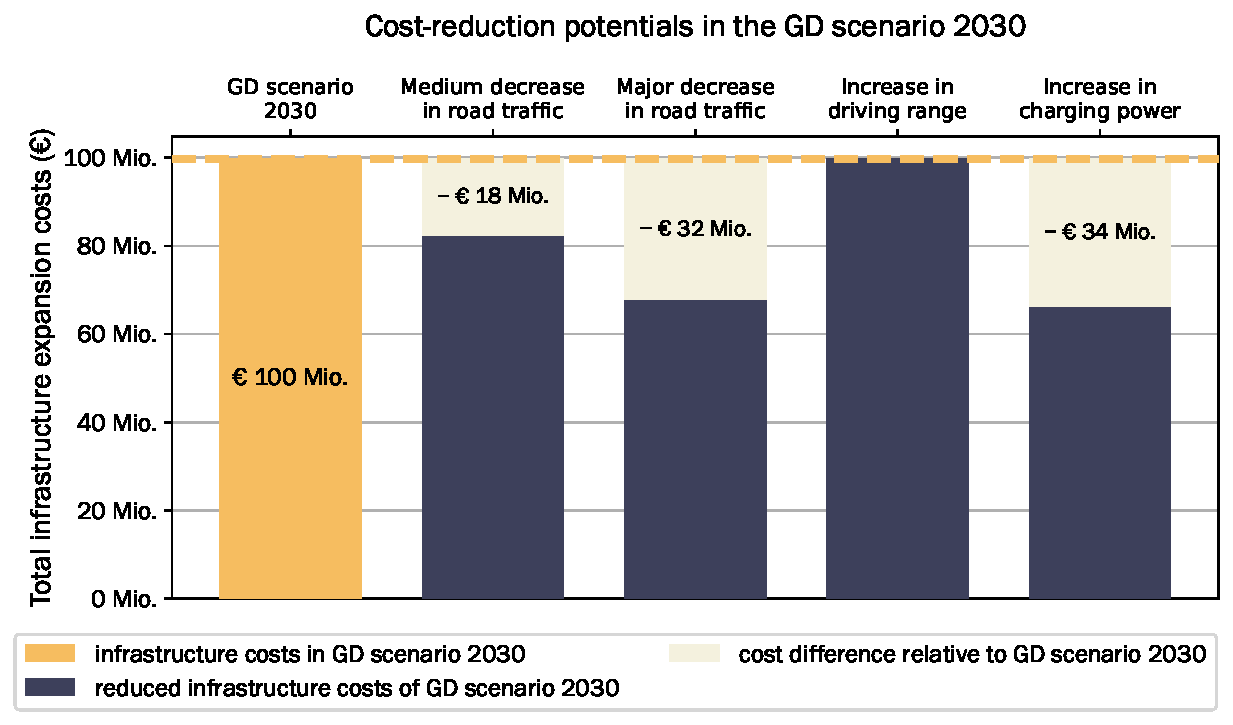
\includegraphics[width=14cm]{images/cost_red.pdf}
\caption{\textbf{Cost reduction potentials in the \textit{Directed Transition} (\textit{DT}) scenario.} (Detailed descriptions of the measures are in Table \ref{tab:cost_red}.) \label{fig:cost_red}}
\end{figure}   
\unskip

\subsection{Sensitivity analyses on the requirements for fast-charging infrastructure }
In the following, the mere infrastructure requirements in 2030 without regards to the charging infrastructure currently in place are analyzed. This is done to better understand how requirements for the fast-charging infrastructure change as a function of technological BEV parameters and in response to growing demand. First, the effect of the average driving range of an average BEV in the Austrian car fleet is observed in the context of the TF scenario during which major developments in battery technology are expected. Second, the change in modeled charging infrastructure depending on the BEV share in the car fleet within the SC scenario, which reflects high societal commitment to BEV uptake, is demonstrated.


\subsubsection{Increasing driving range in the Techno-Friendly scenario}
The driving range is altered between $200$ and $1400km$. Figure \ref{fig:SA_1} presents the changing distribution of the numbers of the charging points at the charging stations and total number of charging stations in response to gradually increasing driving range in the TF scenario. In this figure, the blue boxplots display the distribution of charging points (CP) along the charging stations (CS). The gray dashed line indicates the maximum possible number of  charging points at a charging station which is 34. This is given by the maximum installed capacity of $12MW$ at a charging station. The dark red connected points indicate the total number of charging stations in the modeled charging infrastructure. Table \ref{tab:tech} presents the change in the key parameters for the driving ranges of $200$, $800$ and $1400km$ and gives an impression on how the key parameters of the modeled fast-charging infrastructure change in the course of the conducted sensitivity analysis. Given the assumed development in the TF scenario, the average driving range of BEVs in the Austrian car fleet is projected to be $670km$ by 2030 and reach approximately $1000km$ by around 2040. 

%The secondary x-axis indicates the year during which the respective value resembles the average driving range of BEVs in the Austrian car feet in the TF scenario. 

With the increasing range, energy demand can be shifted further away from the node where it originates, which results in wider solution space during the optimization. Overall, the infrastructure costs stay stable between €71 Mio. and €72 Mio. throughout this parameter alteration. The total number of charging stations decreases from $55$ at $200km$ to a minimum of $38$ at $1100km$. The installed capacity stays constant. Starting at the range of $300km$, fully occupied charging stations occur throughout the sensitivity analysis. Overall the highest costs of investments are at $200km$ and drop\deleted{s} to €71 Mio at the range of $500km$. 

\begin{figure}[H]
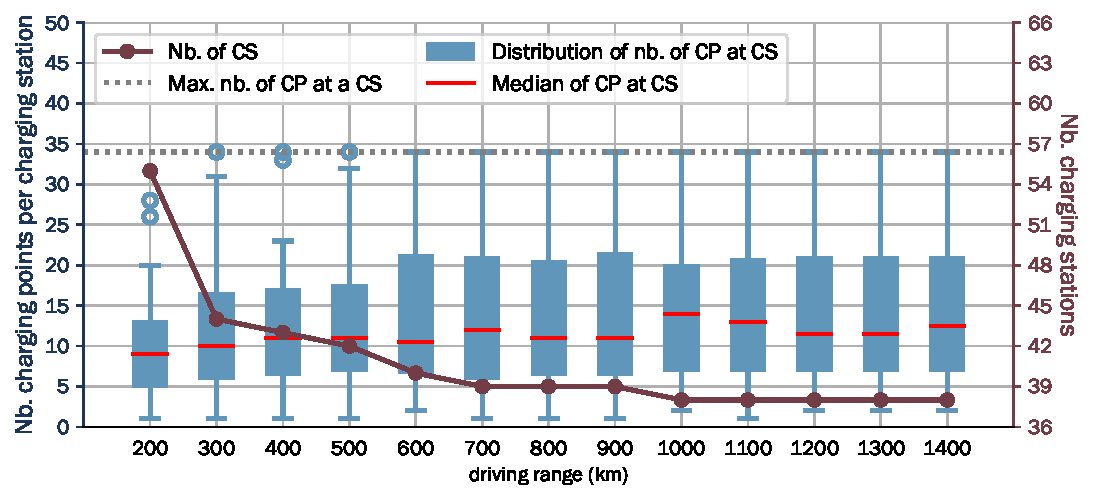
\includegraphics[width=14 cm]{images/range_30.pdf}
\caption{\textbf{Sensitivity analysis on driving range.} Impact of the increase of the driving range of BEVs on the distribution of the number of charging points (\textit{CP}) at charging stations and the total amount of charging stations (\textit{CS}).\label{fig:SA_1}}
\end{figure}   

During this analysis, the model was run for each of the ranges between $200$ and $1400km$ every $100km$ and, therefore, in total, for 13 times. During all of these model runs, at $34$ of all service areas, charging station installations occurred in each of the model runs. The top sub-figure in Figure \ref{fig:constant_cp_1} illustrates these charging stations in black. The bottom illustration shows which of these are currently existing charging stations (in \replaced{bright}{dark} green) and which are not (in red). Overall, $11$ of these $34$ permanent charging stations are existing charging stations. 


\begin{figure}[H]
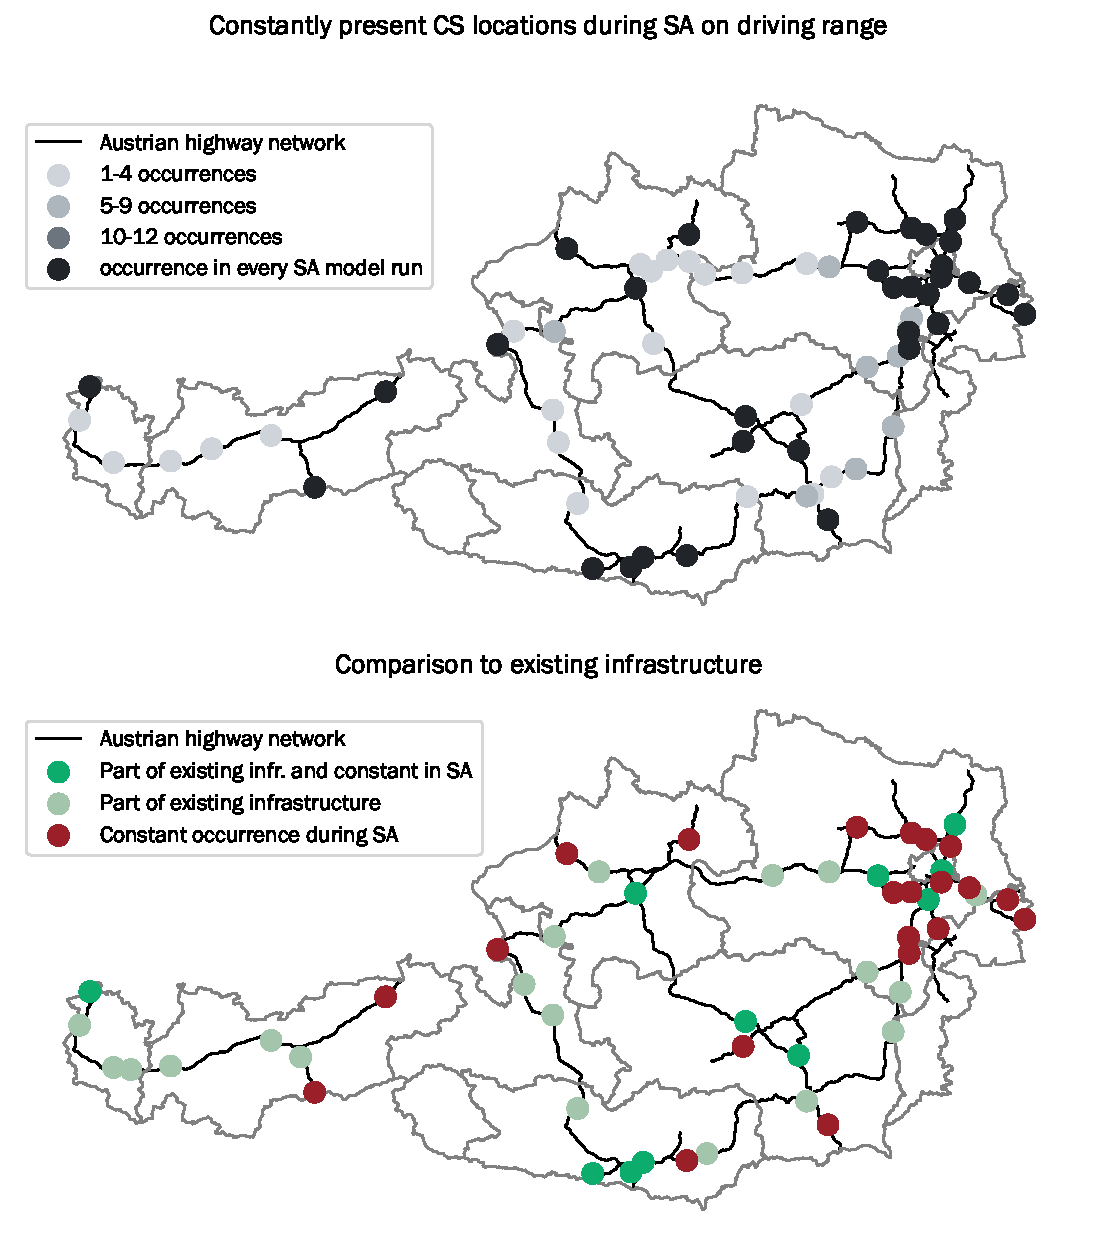
\includegraphics[width=14 cm]{images/steady_CS.pdf}
\caption{\textbf{Frequent charging point allocations.} \textbf{Top:} Visualization of charging stations (\textit{CS}) which occur during the model runs of the sensitivity analysis (\textit{SA}) on BEV driving range. \textbf{Bottom:} Visualization of CS which are constantly present during the SA and are part of the existing infrastructure. \label{fig:constant_cp_1}}
\end{figure}   


\subsubsection{Increasing share of BEVs in the Societal Commitment scenario}
Figure \ref{fig:sa_2_1} presents the results of the sensitivity analysis on the share of BEVs in the Austrian car fleet under the SC scenario for 2030. The top-left sub\added{-}figure presents the total installed capacity of the fast-charging infrastructure as a function of rising share of BEVs. The top-right sub\added{-}figure displays the change in the number of charging stations. Boxplots illustrating the distribution of the number of charging points at charging stations are presented in the bottom-left sub\added{-}figure. The timeline in this figure is projected based on the assumption that as of 2030, all registered cars will be BEVs and a BEV has a lifetime of 10 years which would lead to an Austrian car fleet \replaced{that}{which} is 100 \% electric by 2040. Table \ref{tab:tech} presents the values of parameters describing the key features of modeled infrastructure for the different shares of BEVs, 10\%, 50\% and 100\%.

The required capacity for fast-charging is rising linearly with the share of BEVs. The number of charging stations is significantly increasing between 40\% to 100\%, indicating the requirement for a densification of the fast-charging infrastructure. This effect of densification can be attributed to the increasing amount of fully occupied charging stations which is visible in the bottom left sub-figure of Figure \ref{fig:sa_2_1}. The overall cost increase by a factor of about 10 between 10\% and 100\% share of BEVs, so does the required capacity.


% \begin{itemize}
%     \item linear relation between charging stations and BEV share 
%     \item share of not covered energy stays the same 
%     \item densification due to local constrain on maximum of charging stations at a charging points 
    
% \end{itemize}


\begin{figure}[h]
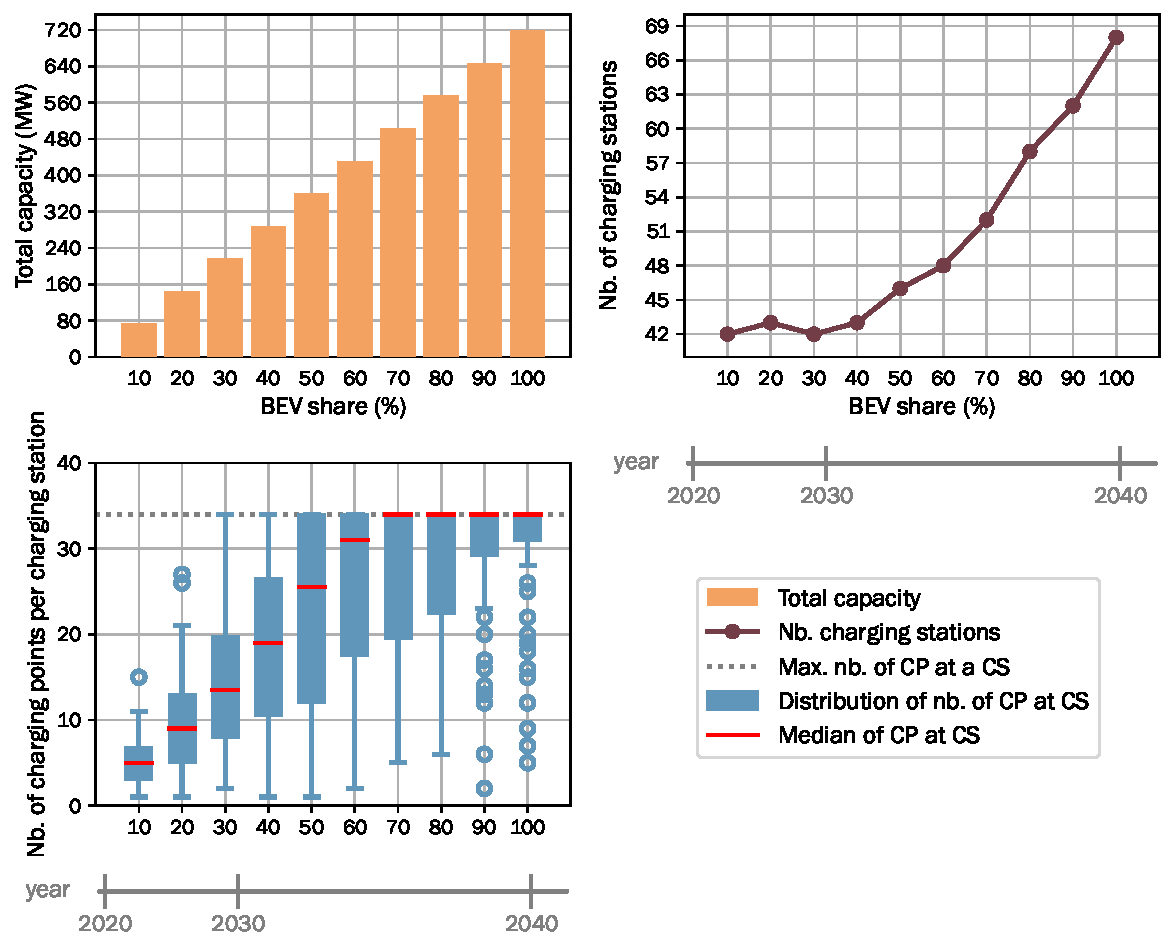
\includegraphics[width=14cm]{images/infr_change.pdf}

\caption{\textbf{Sensitivity analysis of the increasing BEV share.} \textbf{Top-left:} Total required capacity of the fast-charging stations of required charging infrastructure. \textbf{Top-right:}  Number of charging stations (\textit{CS}). \textbf{Bottom-left:} Distribution of the number of charging points (\textit{CP}) at the charging stations. \label{fig:sa_2_1}}
\end{figure}   
\unskip
% Please add the following required packages to your document preamble:
% \usepackage{booktabs}
\begin{table}[H]
\centering
\caption{Key parameters describing the results of the sensitivity analyses on the driving range in the \textit{Techno-Friendly} (\textit{TF}) scenario and share of BEVs in the \textit{Societal Commitment} (\textit{SC}) scenario. \label{tab:tech}}
\newcolumntype{C}{>{\centering\arraybackslash}X}
\begin{tabularx}{\textwidth}{lcccccc}
\toprule
                                                    & \multicolumn{3}{c}{\textbf{driving range $\overline{dist}_{range, BEV}$ (TF)}}  & \multicolumn{3}{c}{\textbf{share of BEV $\epsilon$ (SC)}}\\ \cmidrule(l){2-7} 
                                                              & $200km$                  & $800km$                  & $1400km$   & 10\%              & 50\%              & 100\%                 \\ \midrule
Nb. of charging stations                                             & 55                       & 39                       & 38          & 42                & 46                & 68              \\
Total capacity $(MW)$                                          & 192                      & 192                      & 192     & 73                & 360               & 718                 \\
Total investment costs (€)           & 72 Mio.                  & 71 Mio.                  & 71 Mio.      & 28 Mio.           & 132 Mio.          & 263 Mio.            \\ \bottomrule
\end{tabularx}
\end{table}






%     \item high variation in infrastructure expansion costs in different scenarios; \textrightarrow how technological improvments impact, especially in charging capacity
%     \item Brücke zu \citet{Chakraborty2019}, \citet{Kavianipour2021}: technological developments: range and capacity 
%     \item also cost-reduction potential by modal shift; though it is likely that costs would be allocated in order to support different infrastructure; \textrightarrow co-operational spatial planning; but also behavioral changes not well understood (\citep{Josefina})
%     \item given the topology of the Austrian highway network, there 
%     \item Are there (given the topology), strategic places; such as described by 
%     \item densification of highway network needed or expansion of grid in specific locations (charging parks)
% \end{itemize}

% Authors should discuss the results and how they can be interpreted from the perspective of previous studies and of the working hypotheses. The findings and their implications should be discussed in the broadest context possible. Future research directions may also be highlighted.

% \citet{Carley2016}: suggests investment in  charging equipment, technological development 
% which is in line with 

% \citet{Chakraborty2019}: with longer ranges: infrastructure needs will change


% The high variation required charging infrastructure between the different scenarios indicates the high impact by modal split and 
%%%%%%%%%%%%%%%%%%%%%%%%%%%%%%%%%%%%%%%%%%
\section{Conclusions}

The decarbonization of the passenger sector is an important topic and the diffusion of battery\added{-}electric vehicles (BEVs) is one of the main solutions to counteract the increase in the greenhouse gas emissions in the face of globally growing transport demand. A sufficient and demand-oriented fast-charging infrastructure is needed to support the diffusion of BEVs. The proposed modeling framework reflects the cost-optimal expansion of the fast-charging infrastructure along highways in terms of enabling long-distance travel with BEVs. We present one of the first studies, incorporating the effects of changes in modal split as well as technological developments of BEVs on the design of a fast-charging infrastructure for the future. In our analysis, we observed the effects of charging capacity, as well as, BEV share and the reductions of road traffic load.
% Following the research on the decarbonization of the transport sector, activity reduction and modal shift are important drivers of climate change mitigation and, therefore, need to be accounted for in infrastructure planning. 

% Our findings indicate that a modal shift may reduce charging demand in has the potential of reducing required expansion of the charging infrastructure and, therefore, also associated costs. As the modal shift is also associated with required investments in infrastructure, the awareness of this effect can help in allocating investments cost-optimally.

Particularly, the average charging power level of a BEV is found to have a significant impact on the costs of charging infrastructure installation. With \deleted{the} higher charging power of the BEVs, the required infrastructure expansion at growing BEV share can be reduced. As there is a need to invest in technological developments to overcome the barriers of BEV adoption, we found that these investments can also induce cost-savings in infrastructure expansion. 

% new
In future work, this proposed modeling approach will be compared with flow-based approaches in terms of computation performance and model output. Based on this comparison, the benefits of both approaches could be exploited within the model formulation. Moreover, a verification of the proposed top-down modeling approach could be conducted by testing whether the modeled charging infrastructure is sufficient to meet the fast-charging demand by a traffic flow simulation by means of introducing origin and destination nodes and observing whether the charging demand by all long-distance trips is sufficiently covered and travel times are not substantially prolonged by, e.g., queuing at charging stations. Based on this, the model can be expanded by introducing temporal granularity with regard to charging processes and traffic flow. This can also help in the allocation of charging infrastructure not only in response to yearly peak demand but also in such a way that the profitability of hosting the charging stations is also ensured. Moreover, as it has been found in this paper that technological developments and changes in mobility behavior have significant impact on the required infrastructure but are also quite uncertain in the future, the goal in the future work is to add uncertainty measures that would help in modeling a more realistic charging infrastructure expansion. Building on the insights gained into the impact of technological developments and increasing demand, an extension of the model by the means of the introduction of a temporal dimension in yearly resolution can help model charging infrastructure requirements as a function of changes in technology, modal split and BEV fleet size in time. This could assist policy-makers in making cost-optimal investment decisions throughout the years.

% a further idea of future work 

%The aim of future work is to build on the findings of this paper and introduce geographical differentiation in costs of grid connection. We want to further introduce a temporal dimension to the model which would enable to observe charging infrastructure requirements as a function of changes in technology and modal split in time. This would help in gaining insight into when to make cost-optimal investment decisions. Secondly, this modeled will be applied to large-scale high-level road networks, such as the Trans-European Transport Network, in order to shed light onto needed charging infrastructure expansion across multiple countries, in order to model a charging infrastructure supporting international travel with BEVs. Lastly, as we found that technological developments and changes in mobility behavior have significant impact on required charging infrastructure but are also quite uncertain in the future, the goal in future work is to add uncertainty measures which would help in modeling a more realistic charging infrastructure expansion.   

%future work will include the analysis on not only the cost-optimal allocation of charging infrastructure but also profitable as currently, the model installs infrastructure based on the maximum yearly traffic flow numbers, though this might be timely limited and a charging station could be weakly utilized throughout the rest of the year. Introducing this feature to the model could be achieved, e.g., through the implementation of uncertainties in demand  


% old 

% \begin{itemize}
%     \item Hat sich die MEthode bewert? Habe ich zusätzliche erkenntnisse?
%     \item was bedeuten diese Erkenntnisse jetzt für die Ladeinfr
%     \item Future work 
% \end{itemize}
% This section is not mandatory, but can be added to the manuscript if the discussion is unusually long or complex.



%%%%%%%%%%%%%%%%%%%%%%%%%%%%%%%%%%%%%%%%%%
\vspace{6pt} 

%%%%%%%%%%%%%%%%%%%%%%%%%%%%%%%%%%%%%%%%%%
%% optional
%\supplementary{The following are available online at \linksupplementary{s1}, Figure S1: title, Table S1: title, Video S1: title.}

% Only for the journal Methods and Protocols:
% If you wish to submit a video article, please do so with any other supplementary material.
% \supplementary{The following are available at \linksupplementary{s1}, Figure S1: title, Table S1: title, Video S1: title. A supporting video article is available at doi: link.} 

%%%%%%%%%%%%%%%%%%%%%%%%%%%%%%%%%%%%%%%%%%
\authorcontributions{Conceptualization, A.G., S.Z.-B. and H.A.; methodology, A.G., S.Z.-B. and H.A.; software, A.G.; validation, A.G.; formal analysis, A.G.; investigation, A.G.; resources, A.G.; data curation, A.G.; writing---original draft preparation, A.G.; writing---review and editing, A.G., S.Z.-B. and H.A.; visualization, A.G.; supervision, H.A.; project administration, H.A.; funding acquisition, H.A. All authors have read and agreed to the published version of the manuscript.}

\funding{Open Access Funding by TU Wien Bibliothek.}

\institutionalreview{Not applicable.}

\informedconsent{Not applicable.}

\dataavailability{Data sharing not applicable.} 

\acknowledgments{The authors acknowledge TU Wien Bibliothek for financial support through its Open Access Funding Program.}

\conflictsofinterest{The authors declare no conflict of interest.} 

%% Optional
% \sampleavailability{Samples of the compounds ... are available from the authors.}

%%%%%%%%%%%%%%%%%%%%%%%%%%%%%%%%%%%%%%%%%%
%% Only for journal Encyclopedia
%\entrylink{The Link to this entry published on the encyclopedia platform.}

%%%%%%%%%%%%%%%%%%%%%%%%%%%%%%%%%%%%%%%%%%
%% Optional
% \abbreviations{Abbreviations}{
% The following abbreviations are used in this manuscript:\\

% \noindent 
% \begin{tabular}{@{}ll}
% MDPI & Multidisciplinary Digital Publishing Institute\\
% DOAJ & Directory of open access journals\\
% TLA & Three letter acronym\\
% LD & Linear dichroism
% \end{tabular}}

%%%%%%%%%%%%%%%%%%%%%%%%%%%%%%%%%%%%%%%%%%
%% Optional
% \appendixtitles{no} % Leave argument "no" if all appendix headings stay EMPTY (then no dot is printed after "Appendix A"). If the appendix sections contain a heading then change the argument to "yes".
\appendixstart


\appendix
\section[\appendixname~\thesection]{Supplementary details on methodology and materials \label{app:param}} 
\subsection[\appendixname~\thesubsection]{Determination of average technological parameters for BEVs}

To evaluate the technological parameters of an average battery-electric vehicle (BEV) in the Austrian car fleet, the technological attributes of the most sold car models from the last 3 years were used. These are displayed in Table \ref{tab:top10} with the respective number of sales. Using sale numbers as weights, the weighted averages for the driving range and charging capacity were evaluated.

\begin{table}[H]
\begin{adjustwidth}{-\extralength}{0cm}
\caption{Top 10 sold car models in Austria in 2019-2021 and technical attributes \citep{statista1920, statista21, evdb} (average driving range $\overline{dist}_{range,BEV}$, average charging power $\overline{P}_{charge,BEV}$, average specific energy demand $\overline{d}_{spec,BEV}$). \label{tab:top10} }
\label{tab:app_average}
\resizebox{18.5cm}{!}{%
\begin{tabular}{@{}lcccccc@{}}
\toprule
Car model                        & Sales 2019 & Sales 2020 & Sales 2021 & $\overline{dist}_{range,BEV}$ $(km)$ & \begin{tabular}[c]{@{}c@{}} $\overline{P}_{charge,BEV}$\\ at $\hat{P}_{CP}= 150kW$\\ $(kW)$\end{tabular} & \begin{tabular}[c]{@{}c@{}}$\overline{d}_{spec,BEV}$ \\ highway - cold weather\\ $(kWh/km)$\end{tabular} \\ \midrule
\textit{Tesla Model 3}           & 2342       & 2892       & 3304       & 380                     & 110                                                                                                   & 0.23                                                                                            \\
\textit{Renault Zoe}             & 944        & 2071       & 1778       & 310                     & 41                                                                                                    & 0.22                                                                                            \\
\textit{Kia Niro}                & 1125       & 421        & 924        & 370                     & 77                                                                                                    & 0.24                                                                                            \\
\textit{Hyundai Kona}            & 897        & 861        & -          & 395                     & 64                                                                                                    & 0.28                                                                                            \\
\textit{Audi e-Tron}             & 364        & 782        & 1192       & 285                     & 114                                                                                                   & 0.29                                                                                            \\
\textit{BMW i3}                  & 1191       & 697        & -          & 235                     & 47                                                                                                    & 0.23                                                                                            \\
\textit{VW e-Golf}               & 805        & 401        & -          & 190                     & 39                                                                                                    & 0.24                                                                                            \\
\textit{VW Up!}                  & -          & 376        & -          & 205                     & 30                                                                                                    & 0.22                                                                                            \\
\textit{Mazda MX-30}             & -          & 370        & -          & 170                     & 34                                                                                                    & 0.25                                                                                            \\
\textit{Peugeot 208}             & -          & 355        & -          & 285                     & 78                                                                                                    & 0.23                                                                                            \\
\textit{Hyundai Ioniq}           & 361        & -          & -          & 250                     & 36                                                                                                    & 0.22                                                                                            \\
\textit{Nissan Leaf}             & 557        & -          & -          & 225                     & 40                                                                                                    & 0.23                                                                                            \\
\textit{Tesla Model S}           & 389        & -          & -          & 560                     & 110                                                                                                   & 0.23                                                                                            \\
\textit{VW ID.3}                  & -          & -          & 2361       & 350                     & 85                                                                                                    & 0.23                                                                                            \\
\textit{VW ID.4}                  & -          & -          & 2361       & 400                     & 103                                                                                                   & 0.27                                                                                            \\
\textit{Skoda Enyaq}             & -          & -          & 2208       & 420                     & 103                                                                                                   & 0.26                                                                                            \\
\textit{Fiat 500}                & -          & -          & 1356       & 235                     & 67                                                                                                    & 0.23                                                                                            \\
\textit{Seat Mii}                & -          & -          & 936        & 205                     & 30                                                                                                    & 0.22                                                                                            \\
\textit{Tesla Model Y}           & -          & -          & 921        & 435                     & 108                                                                                                   & 0.24                                                                                            \\ \midrule
\textbf{Weighted average values} &            &            &            & \textbf{340}            & \textbf{81}                                                                                           & \textbf{0.24}                                                                                   \\ \bottomrule
\end{tabular}%
}
\end{adjustwidth}
\end{table}
\subsection[\appendixname~\thesubsection]{Details on the projected developments for 2030 under different scenarios \label{app_2}}

For the quantification of the scenarios used in the analysis, projections on the development of BEV share had to be made. For the \textit{Societal Commitment} and \textit{Techno-Friendly} scenarios an \textit{optimistic} projection was made based on the decarbonization goals for the transport sector in governmental document \enquote{Austria's Mobility Master Plan 2030} \citep{Nachhaltig}. A \textit{pessimistic} projection is made for the \textit{Directed Transition} and \textit{Gradual Development} scenarios based on the trend of new registrations of BEVs in the year between 2018 and 2020. 

\begin{figure}[H]
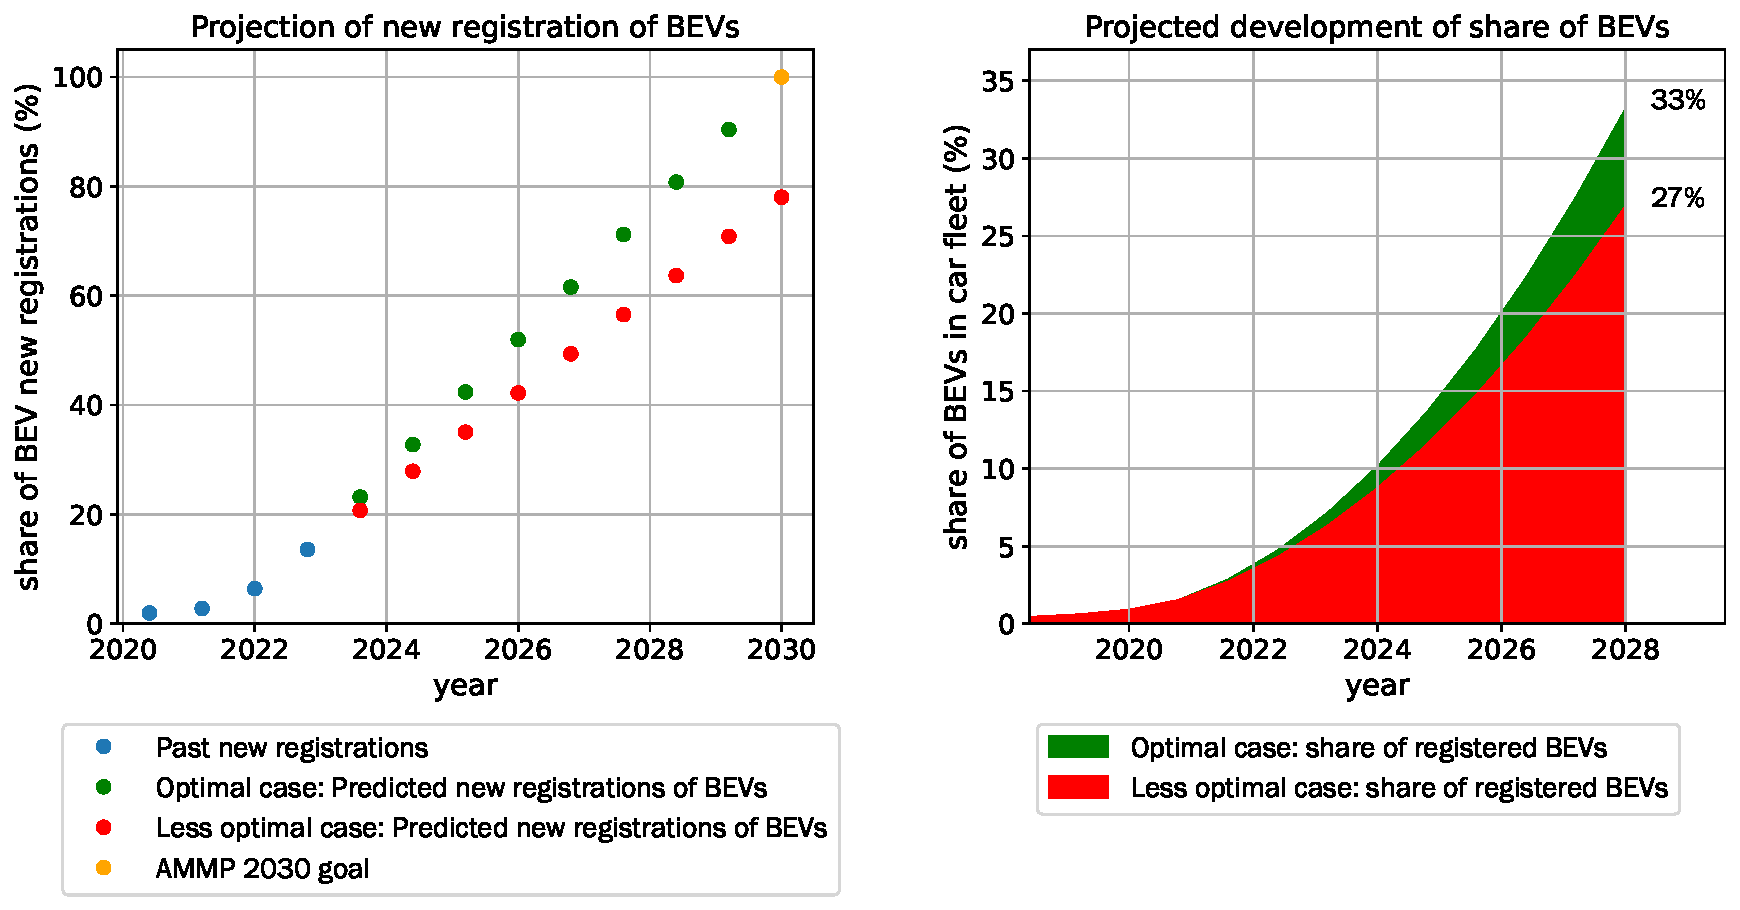
\includegraphics[width=14cm]{images/appendix_img_meth.pdf}
\caption{Projections of linearly increasing new registrations of BEVs (\textbf{left}, \textit{AMMP}=\textit{Austria Mobility Master Plan} \citep{Nachhaltig}) and based on this, developments of share of BEV (\textbf{right}). \label{fig:bev_pen_proj}}
\end{figure}   


\subsection[\appendixname~\thesubsection]{\textcolor{blue}{Details on preparation for the Austrian case study}\label{app_3}}
\textcolor{blue}{
The underlying data pre-processing procedures of this work encompassed the preparation of the graph representation of the Austrian high-level road network and the potential sites for the installment of charging stations. Geographic data representing the Austrian highways and motorways was obtained based on OpenStreetMap data \cite{OpenStreetMap}. For this, all \textit{way} instances with tags \textit{highway='motorway'} and \textit{highway='trunk'} were retrieved and further processed using ArcGIS Pro \cite{desktop2011release} in order to obtain a clean shape representation of the road network, including the representation of both driving directions through parallel lines. Geographic data implying positions of service areas were retrieved using tags \textit{highway='services'} and \textit{highway='rest\_area'}. This geographic information was paired with data on service areas obtained through ASFINAG \cite{asfinagrastanlagen} which provide information on the driving direction a service area is accessible from and on the services offered on-site.
}

% Please add the following required packages to your document preamble:
% \usepackage{booktabs}


% \subsection[\appendixname~\thesubsection]{Input parameters for base case for sensitivity analysis}
% Please add the following required packages to your document preamble:

% The appendix is an optional section that can contain details and data supplemental to the main text---for example, explanations of experimental details that would disrupt the flow of the main text but nonetheless remain crucial to understanding and reproducing the research shown; figures of replicates for experiments of which representative data are shown in the main text can be added here if brief, or as Supplementary Data. Mathematical proofs of results not central to the paper can be added as an appendix.
% \subsection[\appendixname~\thesubsection]{Program implementation}

% The modeling framework described in this paper, including all conducted model calculations were implemented and performed using \texttt{Python 3.8}. Further, \texttt{Gurobi 9.1.2} \citep{gurobi} was used to solve the optimization problem. In order to improve model performance, the mixed integer programming optimality gap (MIPgap) was set the price of one charging pole, $c_Y$.



%%%%%%%%%%%%%%%%%%%%%%%%%%%%%%%%%%%%%%%%%%
\begin{adjustwidth}{-\extralength}{0cm}
%\printendnotes[custom] % Un-comment to print a list of endnotes

\reftitle{References}

% Please provide either the correct journal abbreviation (e.g. according to the “List of Title Word Abbreviations” http://www.issn.org/services/online-services/access-to-the-ltwa/) or the full name of the journal.
% Citations and References in Supplementary files are permitted provided that they also appear in the reference list here. 

%=====================================
% References, variant A: external bibliography
%=====================================
\bibliography{interacttfqsample.bib}

%=====================================
% References, variant B: internal bibliography
%=====================================
% \begin{thebibliography}{999}
% % Reference 1
% \bibitem[Author1(year)]{ref-journal}
% Author~1, T. The title of the cited article. {\em Journal Abbreviation} {\bf 2008}, {\em 10}, 142--149.
% % Reference 2
% \bibitem[Author2(year)]{ref-book1}
% Author~2, L. The title of the cited contribution. In {\em The Book Title}; Editor1, F., Editor2, A., Eds.; Publishing House: City, Country, 2007; pp. 32--58.
% % Reference 3
% \bibitem[Author3(year)]{ref-book2}
% Author 1, A.; Author 2, B. \textit{Book Title}, 3rd ed.; Publisher: Publisher Location, Country, 2008; pp. 154--196.
% % Reference 4
% \bibitem[Author4(year)]{ref-unpublish}
% Author 1, A.B.; Author 2, C. Title of Unpublished Work. \textit{Abbreviated Journal Name} year, \textit{phrase indicating stage of publication (submitted; accepted; in press)}.
% % Reference 5
% \bibitem[Author5(year)]{ref-communication}
% Author 1, A.B. (University, City, State, Country); Author 2, C. (Institute, City, State, Country). Personal communication, 2012.
% % Reference 6
% \bibitem[Author6(year)]{ref-proceeding}
% Author 1, A.B.; Author 2, C.D.; Author 3, E.F. Title of presentation. In Proceedings of the Name of the Conference, Location of Conference, Country, Date of Conference (Day Month Year); Abstract Number (optional), Pagination (optional).
% % Reference 7
% \bibitem[Author7(year)]{ref-thesis}
% Author 1, A.B. Title of Thesis. Level of Thesis, Degree-Granting University, Location of University, Date of Completion.
% % Reference 8
% \bibitem[Author8(year)]{ref-url}
% Title of Site. Available online: URL (accessed on Day Month Year).
% \end{thebibliography}

% If authors have biography, please use the format below
%\section*{Short Biography of Authors}
%\bio
%{\raisebox{-0.35cm}{\includegraphics[width=3.5cm,height=5.3cm,clip,keepaspectratio]{Definitions/author1.pdf}}}
%{\textbf{Firstname Lastname} Biography of first author}
%
%\bio
%{\raisebox{-0.35cm}{\includegraphics[width=3.5cm,height=5.3cm,clip,keepaspectratio]{Definitions/author2.jpg}}}
%{\textbf{Firstname Lastname} Biography of second author}

% For the MDPI journals use author-date citation, please follow the formatting guidelines on http://www.mdpi.com/authors/references
% To cite two works by the same author: \citeauthor{ref-journal-1a} (\citeyear{ref-journal-1a}, \citeyear{ref-journal-1b}). This produces: Whittaker (1967, 1975)
% To cite two works by the same author with specific pages: \citeauthor{ref-journal-3a} (\citeyear{ref-journal-3a}, p. 328; \citeyear{ref-journal-3b}, p.475). This produces: Wong (1999, p. 328; 2000, p. 475)

%%%%%%%%%%%%%%%%%%%%%%%%%%%%%%%%%%%%%%%%%%
%% for journal Sci
%\reviewreports{\\
%Reviewer 1 comments and authors’ response\\
%Reviewer 2 comments and authors’ response\\
%Reviewer 3 comments and authors’ response
%}
%%%%%%%%%%%%%%%%%%%%%%%%%%%%%%%%%%%%%%%%%%
\end{adjustwidth}
\end{document}

